
\documentclass[12pt, a4paper]{report}

\usepackage[utf8]{inputenc}
\usepackage[T1]{fontenc}
\usepackage{times}
\usepackage[margin=1in]{geometry}
\usepackage{setspace}
\usepackage{titlesec}      
\usepackage{graphicx}      
\usepackage{float}         
\usepackage{booktabs}      
\usepackage{longtable}     
\usepackage{array}         
\usepackage{tabularx}      
\usepackage{multirow}      
\usepackage{caption}       
\usepackage{subcaption}    
\usepackage{amsmath, amssymb}
\usepackage{listings}        
\usepackage{tikz}
\usetikzlibrary{shapes.geometric, arrows.meta, positioning, fit, backgrounds, calc}
\usepackage{xcolor}          
\usepackage{hyperref}        
\usepackage{url}             
\usepackage{enumitem}        
\usepackage{fancyhdr}        
\usepackage{tocloft}         
\usepackage{pdfpages}        
\usepackage{mdframed}        
\usepackage{tikz}            

\hypersetup{
    colorlinks=true,
    linkcolor=black,
    citecolor=black,
    urlcolor=blue,
    bookmarksopen=true
}

\onehalfspacing


\titleformat{\chapter}[display]
  {\normalfont\Large\bfseries\centering}
  {CHAPTER \thechapter}{12pt}{\Large\uppercase}
\titlespacing*{\chapter}{0pt}{-20pt}{20pt}

\titleformat{\section}
  {\normalfont\large\bfseries}{\thesection}{1em}{}
\titleformat{\subsection}
  {\normalfont\normalsize\bfseries}{\thesubsection}{1em}{}
\titleformat{\subsubsection}
  {\normalfont\normalsize\itshape}{\thesubsubsection}{1em}{}


\pagestyle{fancy}
\fancyhf{}
\fancyhead[L]{\small\leftmark}
\fancyhead[R]{\small Dept. of Computer Engineering}
\fancyfoot[C]{\thepage}
\renewcommand{\headrulewidth}{0.4pt}
\renewcommand{\footrulewidth}{0pt}


\lstdefinestyle{codestyle}{
    backgroundcolor=\color{gray!5},
    basicstyle=\ttfamily\small,
    breaklines=true,
    frame=single,
    numbers=left,
    numberstyle=\tiny\color{gray},
    keywordstyle=\color{blue}\bfseries,
    commentstyle=\color{green!50!black},
    stringstyle=\color{red!70!black},
    tabsize=4,
    showstringspaces=false
}
\lstset{style=codestyle}


\renewcommand{\cftchapfont}{\bfseries}
\renewcommand{\cftchappagefont}{\bfseries}
\setlength{\cftbeforechapskip}{6pt}


\newcommand{\projecttitle}{X-Sense: Explainable Multimodal Real-Time Sentiment Intelligence System}
\newcommand{\collegename}{Brahma Valley College of Engineering and Research Institute}
\newcommand{\universityname}{Savitribai Phule Pune University}


\begin{document}


\pagenumbering{roman}

\begin{titlepage}
\begin{center}

\vspace*{0.5cm}

{\Large \textbf{A PROJECT REPORT ON}}\\[0.4cm]
{\Large \textbf{\projecttitle}}\\[0.8cm]

{\normalsize SUBMITTED TO THE \MakeUppercase{\universityname}}\\[0.2cm]
{\normalsize IN THE PARTIAL FULFILLMENT OF THE REQUIREMENTS}\\[0.2cm]
{\normalsize FOR THE AWARD OF THE DEGREE}\\[0.2cm]
{\normalsize OF}\\[0.4cm]

{\Large \textbf{BACHELOR OF ENGINEERING}}\\[0.1cm]
{\Large \textbf{(COMPUTER ENGINEERING)}}\\[0.8cm]

{\normalsize \textbf{SUBMITTED BY}}\\[0.4cm]

\begin{tabular}{l l}
{Hase Nayana Dnyandeo} & Seat No.: {B400620202} \\[0.15cm]
{Khanekar Megha Dinkar} & Seat No.: {B400620211} \\[0.15cm]
{Sable Prachi Ashok} & Seat No.: {B400620231} \\[0.15cm]
\end{tabular}

\vspace{0.6cm}

{\normalsize \textbf{UNDER THE GUIDANCE OF}}\\[0.2cm]
{\normalsize {Prof. P.P Kakade}}\\[0.6cm]


\includegraphics[width=2.5cm]{college_logo.jpeg}\\[0.4cm]

{\normalsize \textbf{DEPARTMENT OF COMPUTER ENGINEERING}}\\[0.2cm]
{\normalsize \textbf{\collegename}}\\[0.3cm]

{\normalsize \textbf{\MakeUppercase{\universityname}}}\\[0.2cm]
{\normalsize \textbf{2025--2026}}

\end{center}
\end{titlepage}

\newpage
\thispagestyle{empty}
\begin{center}

\vspace*{0.3cm}

\includegraphics[width=2.5cm]{college_logo.jpeg}\\[0.4cm]

{\large \textbf{CERTIFICATE}}\\[0.5cm]

\end{center}

\noindent
\begin{center}
    This is to certify that the project report entitled\\[0.3cm]
\end{center}

\begin{center}
\textbf{``\projecttitle''}\\[0.3cm]
\textbf{Submitted by}\\[0.3cm]

\begin{tabular}{l l}
{Hase Nayana Dnyandeo} & Seat No.: {B400620202} \\[0.15cm]
{Khanekar Megha Dinkar} & Seat No.: {B400620211} \\[0.15cm]
{Sable Prachi Ashok} & Seat No.: {B400620231} \\[0.15cm]
\end{tabular}
\end{center}

\vspace{0.3cm}
\noindent
are bonafide students of this institute and the work has been carried out by them under the supervision of \textbf{{Prof. P.P. Kakade}} and it is approved for the partial fulfillment of the requirement of \textbf{\universityname}, for the award of the degree of \textbf{Bachelor of Engineering} (Computer Engineering).

\vfill

\noindent
\begin{tabular}{@{}p{0.48\textwidth}p{0.48\textwidth}@{}}
\textbf{{Prof. P.P. Kakade}} & \textbf{{Prof. P.P. Kakade}} \\
Guide & Head \\
Department of Computer Engineering & Department of Computer Engineering \\
\end{tabular}

\vfill

\noindent
\begin{tabular}{@{}p{0.48\textwidth}p{0.48\textwidth}@{}}
\textbf{{Dr.H.N.Kudal}} & \textbf{Project External} \\
Principal & \\
\end{tabular}

\vfill

\begin{center}
{\normalsize \textbf{DEPARTMENT OF COMPUTER ENGINEERING}}\\[0.2cm]
{\normalsize \textbf{\collegename}}\\[0.3cm]
{\normalsize \textbf{\MakeUppercase{\universityname}}}\\[0.2cm]
{\normalsize \textbf{2025--2026}}
\end{center}

\newpage
\chapter*{Declaration}
\addcontentsline{toc}{chapter}{Declaration}

We, the undersigned, hereby declare that the project entitled \textbf{``\projecttitle''} submitted to the Department of Computer Engineering in partial fulfillment of the requirements for the award of the Degree of Bachelor of Engineering is a record of original work carried out by us under the guidance of \textbf{{Prof. P.P. Kakade}}.

We further declare that this project or any part thereof has not been submitted for the award of any degree, diploma, or any other academic qualification at any university or institution. The work presented in this project is genuine and has not been copied from any other source without proper reference and acknowledgment.

All information and data used in this project have been collected and processed in good faith. Any resemblance to other published work is purely coincidental and unintentional.

\vspace{1.5cm}

\vspace{0.8cm}
\begin{flushright}
\begin{tabular}{l l}
{Hase Nayana Dnyandeo} & Seat No.: {B400620202} \\[0.15cm]
{Khanekar Megha Dinkar} & Seat No.: {B400620211} \\[0.15cm]
{Sable Prachi Ashok} & Seat No.: {B400620231} \\[0.15cm]
\end{tabular}

\vspace{1.5cm}
Date: \underline{\hspace{4cm}} \hspace{1cm} Place: \underline{\hspace{4cm}}
\end{flushright}
\newpage
\chapter*{Acknowledgement}
\addcontentsline{toc}{chapter}{Acknowledgement}

We take this opportunity to express our heartfelt gratitude to all those who have contributed to the successful completion of this project.

First and foremost, we extend our sincere thanks to our project guide \textbf{{Prof. P.P. Kakade}} for their invaluable guidance, constant encouragement, constructive suggestions, and continuous support throughout the development of this project. Their expertise and insight proved instrumental in shaping this work.

We are deeply grateful to \textbf{{Prof. P.P. Kakade}}, Head of the Department of Computer Engineering, for providing us with the necessary infrastructure, resources, and an environment conducive to research and development. We also thank the entire faculty and staff of the Computer Engineering department for their help and encouragement throughout our academic journey.

We would like to acknowledge the open-source communities behind the tools and frameworks that made this project possible, including \textbf{Hugging Face}, \textbf{OpenAI}, \textbf{Flask}, \textbf{React}, and the many contributors whose libraries we have relied upon. Their dedication to open and accessible technology has significantly lowered the barrier for academic and research projects like ours.

Finally, we express our deepest gratitude to our families and friends for their endless patience, moral support, and encouragement. This project would not have been possible without their unwavering belief in our abilities.

\vspace{1.5cm}
\begin{flushright}
\textbf{{{Hase Nayana Dnyandeo}}}\\
\textbf{{Khanekar Megha Dinkar}}\\
\textbf{{Sable Prachi Ashok}}\\[0.5cm]
Department of Computer Engineering\\
\collegename\\
\end{flushright}

\newpage
\chapter*{Abstract}
\addcontentsline{toc}{chapter}{Abstract}

Sentiment analysis is a well-established area of natural language processing that aims to identify and categorize the emotional tone embedded in textual data. However, modern-day communication extends far beyond plain text. Users express opinions and emotions through images, audio recordings, video clips, and social media posts. Traditional sentiment analysis systems, which operate exclusively on text, are therefore limited in their ability to comprehensively capture the sentiment present in real-world content.

\textbf{X-Sense} is an Explainable Multimodal Real-Time Sentiment Intelligence System that bridges this gap by providing a unified platform capable of processing text, image, audio, video, and URL-based social media content. The system performs language detection, automatic translation of non-English text into English, and then applies transformer-based deep learning models to predict sentiment with high accuracy. An explainability layer, powered by \textbf{LIME} (Local Interpretable Model-agnostic Explanations), generates word-level and feature-level justifications for each prediction, enabling users to understand the reasoning behind the model output rather than relying on a black-box score.

The backend is built using the Python \textbf{Flask} framework and exposes a RESTful API consumed by a \textbf{React}-based frontend. Sentiment analysis for text leverages the \textbf{Hugging Face Transformers} library, which provides access to pre-trained transformer models fine-tuned for emotion-first sentiment classification. Audio and video content is processed by first transcribing speech using \textbf{OpenAI Whisper} and then analyzing the transcribed text. Image sentiment is evaluated through a combination of heuristic feature extraction using \textbf{OpenCV} and optional zero-shot classification using CLIP-based models.

Social media and web URL inputs are handled by a dedicated scraping module that extracts textual content from public pages, Twitter/X posts, and Instagram embeds. Each analysis is persisted in a \textbf{SQLite} database, enabling users to maintain a full history of their analyses. The system further supports the generation of downloadable PDF reports summarizing all analysis results. A dashboard provides aggregated statistics including overall sentiment distributions, input type breakdowns, and historical trends.

The project successfully demonstrates the integration of full-stack web development, machine learning inference, natural language processing, computer vision, and explainable AI into a single cohesive platform.

\vspace{0.5cm}
\noindent\textbf{Keywords:} Sentiment Analysis, Explainable AI, LIME, Multimodal Analysis, Natural Language Processing, Transformers, Hugging Face, OpenAI Whisper, Flask, React, Image Sentiment, Audio Sentiment, Social Media Analysis.

\newpage
\tableofcontents


\newpage
\listoffigures
\addcontentsline{toc}{chapter}{List of Figures}


\newpage
\listoftables
\addcontentsline{toc}{chapter}{List of Tables}


\newpage
\pagenumbering{arabic}

\newpage
\thispagestyle{empty}

\vspace*{\fill}
\begin{center}
{\Huge \textbf{Chapter 1}}\\[1cm]
{\Huge \textbf{Introduction}}
\end{center}
\vspace*{\fill}

\stepcounter{chapter}
\addcontentsline{toc}{chapter}{\protect\numberline{\thechapter}Introduction}
\markboth{CHAPTER 1. INTRODUCTION}{}
\newpage

The rapid proliferation of digital communication channels has fundamentally transformed the way human beings express thoughts, emotions, and opinions. From microblogging platforms such as Twitter to multimedia-rich applications such as Instagram and YouTube, people continuously generate content that carries embedded sentiment. Businesses, governments, researchers, and social media analysts have a growing need to understand the emotional tone of this content in real time to make informed decisions. Sentiment analysis --- the computational study of opinions, sentiments, and subjectivity --- has emerged as a critical tool for fulfilling this need.

Traditional sentiment analysis systems were developed primarily for text-based content. These systems typically relied on rule-based lexicon matching or simple machine learning classifiers trained on annotated corpora. While effective in constrained laboratory settings, such systems suffer from significant limitations when applied to real-world use cases. They struggle with sarcasm and irony, perform poorly on mixed-language or code-switched content, and cannot process the rich multimodal information present in images, audio recordings, and video streams.

The challenge is not merely technical but also conceptual. Modern communication is inherently multimodal. A tweet may contain text and an image, each potentially conveying different or complementary sentiment signals. A product review may include a video where the speaker's tone of voice and facial expression add nuance that text alone cannot capture. An Instagram post may combine a caption with a visually expressive photograph. A complete sentiment intelligence system must be capable of ingesting and reasoning about all these modalities simultaneously.

\textbf{X-Sense} has been designed to address these challenges. It is an Explainable Multimodal Real-Time Sentiment Intelligence System that accepts five distinct input modalities: plain text, image files, audio recordings, video files, and social media or web URLs. For each input, the system performs a full analysis pipeline involving preprocessing, language detection, translation when necessary, sentiment classification using deep learning models, and the generation of human-interpretable explanations. The output includes a sentiment label, confidence scores for each sentiment class, a word-level or feature-level explanation, a list of influential keywords, and a downloadable PDF report.

The design of X-Sense is guided by three core principles:

\begin{itemize}[noitemsep, leftmargin=1.5em]
    \item \textbf{Comprehensiveness} --- handles all major input modalities and supports multilingual content.
    \item \textbf{Explainability} --- every prediction is accompanied by a clear and interpretable justification.
    \item \textbf{Usability} --- accessible to non-technical users through a clean web interface while also exposing a RESTful API for programmatic integration.
\end{itemize}

The system is built using a modern technology stack. The backend is implemented in Python using \textbf{Flask}. The frontend is implemented in \textbf{React 18}, paired with \textbf{Vite} for fast builds and \textbf{Chart.js} for interactive data visualizations. The machine learning components draw on the \textbf{Hugging Face Transformers} library for text sentiment classification, \textbf{OpenAI Whisper} for speech-to-text transcription, \textbf{OpenCV} and \textbf{Pillow} for image processing, and \textbf{LIME} for explainability. Data persistence is handled by \textbf{SQLite} through the \textbf{Flask-SQLAlchemy} ORM.

\section{Motivation}

The motivation for developing X-Sense arises from several observations about the current state of sentiment analysis technology and its application in practice.

\textbf{First}, the vast majority of commercially available and open-source sentiment analysis tools are text-only. Tools such as VADER, TextBlob, and basic transformer fine-tuned models accept raw text as input and return a polarity score or label. While useful in simple use cases such as analyzing customer reviews written in English, these tools fail as soon as the input deviates from their expected format.

\textbf{Second}, even among systems that do perform reasonable sentiment analysis, the lack of explainability is a persistent problem. Users are often presented with a label such as \textit{Positive} or a numeric score such as \textit{0.87} without any indication of which parts of the input drove the prediction. This black-box behavior is unacceptable in high-stakes applications such as content moderation.

\textbf{Third}, multilingual content presents a significant barrier. The majority of sentiment models are trained on English corpora and perform poorly on other languages. In a globally connected world, a sentiment analysis tool that works only on English is fundamentally limited in its reach.

\textbf{Fourth}, the storage and retrieval of past analyses is rarely supported by existing tools. Each analysis is a one-time operation with no persistence, no history, and no ability to generate reports.

X-Sense was built to address all four of these motivations: by supporting five input modalities, integrating LIME-based explainability, incorporating language detection and translation, and persisting all analyses with full metadata and PDF report generation.

\section{Problem Statement}

Given the limitations of existing sentiment analysis tools, there is a clear need for a comprehensive sentiment intelligence system that satisfies the following requirements:

\begin{enumerate}[noitemsep, leftmargin=2em]
    \item The system must support multiple input modalities including text, images, audio, video, and URLs, processing each through an appropriate analysis pipeline.
    \item The system must detect the language of textual content automatically and translate non-English content to English before analysis, preserving the original input for display.
    \item The system must provide explainable predictions that identify which features of the input contributed most to the predicted sentiment, enabling human oversight and verification.
    \item The system must persist all analysis results in a structured database and allow users to retrieve their full analysis history.
    \item The system must generate downloadable PDF reports summarizing the analysis, suitable for documentation and sharing.
    \item The system must provide an authenticated web-based user interface accessible to non-technical users while also exposing a RESTful API for programmatic access.
    \item The system must include a dashboard that presents aggregated statistics over all analyses performed by a given user.
\end{enumerate}

The problem is therefore not merely to build another sentiment classifier, but to build a complete sentiment intelligence platform that integrates multiple technologies into a unified, user-friendly, and trustworthy system.

\section{Objectives}

The primary objectives of the X-Sense project are as follows:

\begin{itemize}[noitemsep, leftmargin=1.5em]
    \item Design and implement a multimodal sentiment analysis pipeline capable of processing text, images, audio, video, and web URLs.
    \item Integrate transformer-based sentiment classification models from Hugging Face.
    \item Implement automatic language detection using \texttt{langdetect} and translation using \texttt{deep\_translator}.
    \item Integrate OpenAI Whisper for high-accuracy speech-to-text transcription.
    \item Implement image sentiment analysis using heuristic feature extraction and optional CLIP-based zero-shot classification.
    \item Build a web scraping module that extracts textual content from social media posts and public web pages.
    \item Integrate LIME to generate word-level explanations for each text-based prediction.
    \item Design and implement a SQLite-backed persistence layer using SQLAlchemy.
    \item Build a Flask-based RESTful API with JWT-based authentication.
    \item Build a React-based frontend with a dashboard and results visualization using Chart.js.
    \item Implement PDF report generation using the \texttt{fpdf2} library.
\end{itemize}

\section{Scope of the Project}

The scope of X-Sense encompasses the design, development, testing, and documentation of a full-stack multimodal sentiment analysis platform, covering the following areas:

\begin{itemize}[noitemsep, leftmargin=1.5em]
    \item \textbf{Text Analysis:} The system processes plain text input of any length in any supported language. It detects the language, translates if necessary, applies the sentiment classification model, generates LIME-based explanations, and extracts influential keywords. Over 100 languages are supported collectively by \texttt{langdetect} and \texttt{deep\_translator}.
    \item \textbf{Image Analysis:} The system accepts image files in PNG, JPEG, and BMP formats. It applies heuristic analysis based on brightness, color warmth, texture complexity, and face detection. When optional CLIP integration is enabled, it also applies zero-shot visual sentiment classification.
    \item \textbf{Audio and Video Analysis:} The system accepts audio files (MP3, WAV) and video files (MP4). Audio is transcribed using OpenAI Whisper, and the transcribed text is analyzed as standard text. For video, optional frame-by-frame visual sentiment analysis is performed in addition to audio transcription, with scores fused to produce a combined result.
    \item \textbf{URL Analysis:} The system accepts URLs pointing to public web pages, Twitter/X posts, and Instagram posts. It extracts textual content from each source and analyzes each piece of content independently, returning per-item and aggregate results.
\end{itemize}

The scope does \textbf{not} include real-time streaming analysis, integration with proprietary social media APIs beyond publicly available credentials, or the training of custom machine learning models from scratch.

\section{Organization of the Report}

The remainder of this report is organized as follows:

\begin{itemize}[noitemsep, leftmargin=1.5em]
    \item \textbf{Chapter 2:} Literature Survey --- Reviews major approaches, techniques, and systems in sentiment analysis.
    \item \textbf{Chapter 3:} Software Requirements Specification --- Presents functional and non-functional requirements, hardware and software specifications.
    \item \textbf{Chapter 4:} Design --- Describes system architecture, data flow diagrams, UML diagrams, and the processing pipeline.
    \item \textbf{Chapter 5:} Implementation --- Details the backend, analysis pipeline, frontend, and database implementation with screenshots.
    \item \textbf{Chapter 6:} Conclusion --- Summarizes contributions and outlines future work.
    \item \textbf{Chapter 7:} Research Paper --- A formal paper summarizing the system and its experimental evaluation.
    \item \textbf{Chapter 8:} References --- Lists all cited works and documentation.
    \item \textbf{Chapter 9:} Members Details --- Lists team members and their individual contributions.
\end{itemize}

\newpage
\thispagestyle{empty}

\vspace*{\fill}
\begin{center}
{\Huge \textbf{Chapter 2}}\\[1cm]
{\Huge \textbf{Literature Survey}}
\end{center}
\vspace*{\fill}

\stepcounter{chapter}
\addcontentsline{toc}{chapter}{\protect\numberline{\thechapter}Literature Survey}
\markboth{CHAPTER 2. LITERATURE SURVEY}{}
\newpage

The field of sentiment analysis, also widely referred to as opinion mining, has a rich history spanning several decades. As digital communication has evolved from simple text to rich multimodal media, the techniques used to extract subjective information have similarly advanced. This chapter presents a comprehensive review of the major approaches, techniques, and systems that have shaped the current state of the art, and situates X-Sense within this broader academic and technological context.

\section{Lexicon-Based Approaches}

The earliest sentiment analysis systems relied heavily on manually or semi-automatically constructed lexicons --- dictionaries that mapped words or phrases to specific polarity scores. Systems such as \textbf{SentiWordNet}, which built upon the WordNet lexical database to assign sentiment scores to synsets (cognitive synonyms), provided the foundational tools for early researchers. Similarly, \textbf{AFINN} and \textbf{VADER} (Valence Aware Dictionary and sEntiment Reasoner) assigned positive, negative, and neutral weights to individual words, incorporating grammatical heuristics to adjust scores based on punctuation or capitalization.

While lexicon-based methods are computationally lightweight and highly interpretable, they suffer from strict limitations. They struggle with context dependence, sarcasm, and domain-specific vocabulary. A word like "unpredictable" might carry a positive valence in a movie review but a strongly negative valence in an automotive steering review. 

Turney (2002) proposed one of the first unsupervised learning approaches to bridge this gap, using point-wise mutual information (PMI) to assess the semantic orientation of phrases extracted from reviews by measuring their co-occurrence with seed words like "excellent" or "poor." Shortly after, Pang, Lee, and Vaithyanathan (2002) demonstrated that supervised machine learning classifiers trained on bag-of-words features could consistently outperform lexicon-based baselines, marking a definitive shift toward data-driven approaches.

\section{Machine Learning Approaches}

Following the foundational work of Pang et al., a large body of research explored the application of classical machine learning algorithms to sentiment analysis. Researchers moved beyond simple boolean term presence, employing Term Frequency-Inverse Document Frequency (TF-IDF) to appropriately weight words based on their rarity across a corpus.

Algorithms such as \textbf{Support Vector Machines (SVMs)}, Naive Bayes classifiers, Maximum Entropy models, and Logistic Regression became the industry standard. SVMs, in particular, proved highly effective in high-dimensional sparse text spaces. Researchers also experimented with structural features, incorporating n-grams, part-of-speech (POS) tags, and dependency parsing to capture negation (e.g., "not good") and intensification.

However, feature engineering remained a massive bottleneck. The effectiveness of these models was bounded by the quality of manually crafted features, and they struggled to capture the deeper, compositional semantics of human language. Socher et al. (2013) addressed this by introducing the \textbf{Stanford Sentiment Treebank} and demonstrating that recursive neural networks applied to constituency parse trees could capture fine-grained sentiment at the phrase level, effectively modeling how the sentiment of a sentence is compositionally constructed from its constituent words.

\section{Deep Learning and Dense Embeddings}

The advent of deep learning brought significant improvements, primarily driven by the transition from sparse representations (bag-of-words) to dense vector representations known as word embeddings. Models like \textbf{Word2Vec} (Mikolov et al., 2013) and \textbf{GloVe} (Pennington et al., 2014) mapped words into continuous vector spaces where semantic similarities were preserved geometrically.

Armed with these dense representations, researchers applied deep neural architectures to sequence modeling. \textbf{Recurrent Neural Networks (RNNs)} and their more stable variants, \textbf{Long Short-Term Memory (LSTM)} networks and Gated Recurrent Units (GRUs), were applied to sentiment classification. These models could process text sequentially, retaining a "memory" of previous words, which was crucial for resolving long-term dependencies in sentences. 

Concurrently, Kim (2014) showed that \textbf{Convolutional Neural Networks (CNNs)}, typically used in computer vision, could be applied directly to word embedding matrices. By using sliding 1D convolutional filters of various window sizes, CNNs could effectively capture local n-gram features, achieving strong results on sentence-level sentiment classification with significantly faster training times than LSTMs.

The introduction of attention mechanisms by Bahdanau et al. (2015) further improved model performance. By allowing the network to dynamically "attend" to the most relevant hidden states of the input sequence during prediction, attention mechanisms not only boosted accuracy but also provided a rudimentary form of interpretability via attention weights.

\section{Transformer-Based Models}

The publication of the \textbf{Transformer} architecture by Vaswani et al. (2017) and the subsequent introduction of \textbf{BERT} (Bidirectional Encoder Representations from Transformers) by Devlin et al. (2018) marked a paradigm shift in Natural Language Processing. Transformers eliminated the sequential processing bottleneck of LSTMs by relying entirely on the self-attention mechanism, formally defined as:
$$ \text{Attention}(Q, K, V) = \text{softmax}\left(\frac{QK^T}{\sqrt{d_k}}\right)V $$
where $Q$, $K$, and $V$ represent the query, key, and value matrices, respectively, and $d_k$ is the scaling factor.

Pre-trained on massive text corpora using masked language modeling, BERT and its successors --- \textbf{RoBERTa}, \textbf{XLNet}, \textbf{ALBERT}, and \textbf{DistilBERT} --- demonstrated that fine-tuning a pre-trained language model on a task-specific dataset could achieve state-of-the-art performance across nearly all NLP benchmarks. \textbf{RoBERTa} (Liu et al., 2019) improved upon BERT by training on more data with a larger batch size and removing the next-sentence prediction objective, resulting in more robust downstream performance. 

X-Sense heavily leverages this architecture. It uses Hugging Face Transformers to access fine-tuned, quantized transformer checkpoints for emotion-first sentiment classification, mapping granular emotional categories (e.g., joy, anger, sadness, surprise, fear) into aggregate positive, negative, and neutral distributions.

\section{Explainable AI (XAI) and LIME}

As deep learning models grew in complexity, they became opaque "black boxes." This lack of transparency poses significant challenges for user trust and regulatory compliance (such as the GDPR's "Right to Explanation"). To address this, the field of Explainable AI (XAI) has rapidly expanded.

Ribeiro, Singh, and Guestrin (2016) introduced \textbf{LIME} (Local Interpretable Model-agnostic Explanations), a technique that explains individual predictions of any complex classifier by approximating its behavior locally. LIME perturbs the specific input --- for instance, by randomly masking words in a text snippet --- and observes the resulting changes in the model's confidence. It then fits a simple, interpretable linear surrogate model (like Ridge Regression) to this locally generated dataset. The resulting coefficients provide intuitive, word-level importance weights.

Lundberg and Lee (2017) later introduced \textbf{SHAP} (SHapley Additive exPlanations), a method grounded in cooperative game theory that assigns a unified measure of feature importance. While SHAP guarantees theoretical consistency, it is computationally expensive for high-dimensional data. X-Sense therefore prioritizes LIME as its primary explainability engine to maintain real-time responsiveness, providing users with immediate visual feedback on which textual elements drove the AI's conclusion.

\section{Multimodal Sentiment Analysis}

Human communication is inherently multimodal; sentiment is conveyed not just through text, but via tone of voice, facial expressions, and surrounding context. Research in multimodal sentiment analysis has grown substantially, driven by standardized datasets such as \textbf{CMU-MOSI} and \textbf{CMU-MOSEI}. 

Early systems relied on \textit{late fusion} (decision-level fusion), where unimodal models were trained independently, and their outputs were averaged or passed to a secondary classifier. Later work explored \textit{early fusion} (feature-level fusion) and sophisticated attention-based mechanisms. Zadeh et al. (2017) proposed the \textbf{Tensor Fusion Network}, which explicitly models unimodal, bimodal, and trimodal interactions by computing the outer product of unimodal representations.

X-Sense adopts a pragmatic, highly scalable approach to multimodal fusion. It processes each modality through its own specialized, state-of-the-art pipeline and combines the resulting confidence scores through a customizable, weighted late-fusion mechanism. This prioritizes system modularity, allowing individual models to be upgraded independently without retraining a massive joint-representation space.

\section{Speech and Audio Sentiment Analysis}

Speech-based sentiment analysis traditionally focuses on extracting acoustic features --- such as Mel-Frequency Cepstral Coefficients (MFCCs), pitch variations, and energy dynamics (prosody) --- to detect emotional arousal and valence. 

However, modern systems frequently combine acoustic features with high-fidelity Automatic Speech Recognition (ASR). By transcribing speech to text, the immense power of NLP transformers can be brought to bear on the spoken word. \textbf{OpenAI Whisper} (2022), an encoder-decoder Transformer trained on 680,000 hours of diverse multilingual speech data, achieves near-human-level robustness against background noise and accents. X-Sense implements Whisper as its primary speech ingestion engine, bridging the gap between raw audio signals and its core transformer-based text analyzer.

\section{Image Sentiment Analysis}

Visual sentiment analysis aims to identify the affective state evoked by an image. Early research relied on low-level artistic and heuristic features like color harmony, saturation, rule-of-thirds, and visual complexity. Later, Convolutional Neural Networks (like VGG-16 and ResNet) were fine-tuned on large-scale datasets for Facial Emotion Recognition (FER) and visual sentiment prediction.

More recently, foundation models have unified vision and language. \textbf{CLIP} (Contrastive Language-Image Pre-Training) by Radford et al. (2021), trained on 400 million image-text pairs, learns a joint embedding space that enables zero-shot image classification. By computing cosine similarity between an image's vector and text prompts (e.g., "a joyful scene", "a gloomy atmosphere"), CLIP can infer sentiment without explicit task-specific training. X-Sense provides an architecture that supports CLIP for deep semantic image analysis, while maintaining heuristic analysis (brightness, warmth, standard deviation) and traditional face-detection algorithms as a computationally lightweight, robust fallback.
\newpage
\thispagestyle{empty}

\vspace*{\fill}
\begin{center}
{\Huge \textbf{Chapter 3}}\\[1cm]
{\Huge \textbf{Software Requirements Specification}}
\end{center}
\vspace*{\fill}

\stepcounter{chapter}
\addcontentsline{toc}{chapter}{\protect\numberline{\thechapter}Software Requirements Specification}
\markboth{CHAPTER 3. SOFTWARE REQUIREMENTS SPECIFICATION}{}
\newpage

A Software Requirements Specification (SRS) is a foundational document in the software engineering lifecycle. It establishes a precise, verifiable, and complete description of what a system must do, how it must perform, and the environment in which it must operate. For a complex, multi-layered system such as X-Sense --- which integrates full-stack web development, multiple machine learning pipelines, explainable AI, multilingual NLP, and real-time data persistence --- a rigorous SRS is especially critical. It serves as the shared contract between developers, testers, and evaluators, ensuring that every component of the platform is built to a known and agreed-upon standard.

This chapter presents a comprehensive specification for the X-Sense platform. It is organized as follows: Section 3.1 details the software technology stack. Section 3.2 describes the hardware requirements for both development and production environments. Section 3.3 catalogues all functional requirements. Section 3.4 enumerates non-functional requirements covering performance, security, and maintainability. Section 3.5 presents the use case diagram. Sections 3.6 and 3.7 document the advantages and limitations of the system. Section 3.8 surveys practical application domains.

\section{Software Specification}

The X-Sense system is built entirely on a modern, open-source software stack. The selection of each technology was guided by three criteria: maturity and community support, suitability for the specific task, and compatibility with the broader scientific Python ecosystem. The technology stack is deliberately decoupled, with the frontend, backend, machine learning layer, and database each independently replaceable without affecting the others.

\subsection{Frontend Technologies}

The client-facing interface is implemented as a Single Page Application (SPA) using \textbf{React 18}, the most widely adopted JavaScript UI library. React's component-based architecture allows the complex multi-tab analysis interface to be constructed from reusable, independently testable units. The project is scaffolded with \textbf{Vite}, a next-generation build tool that provides sub-second hot module replacement during development and highly optimized production bundles. Client-side navigation between protected and public routes is handled by \textbf{React Router v6}, which provides a declarative routing model with built-in support for nested layouts and route guards. Interactive data visualizations on the dashboard and results pages are powered by \textbf{Chart.js 3.x}, which offers a lightweight and accessible set of chart types including doughnut, bar, and line charts.

\subsection{Backend Technologies}

The server-side API is implemented using \textbf{Flask 3.x}, a lightweight Python WSGI microframework that provides a minimal but extensible foundation for building RESTful services. Flask's blueprint system is used to organize the API into three logically separated modules --- authentication, analysis, and dashboard --- each independently testable. \textbf{Flask-CORS} is configured to permit cross-origin requests from the React development server during development, and from the production domain in deployment. Object-relational mapping and database session management are handled by \textbf{Flask-SQLAlchemy 3.x}, which abstracts the underlying database engine and enables transparent migration from SQLite in development to MySQL or PostgreSQL in production.

\subsection{Machine Learning and AI Technologies}

The machine learning stack is the intellectual core of the platform. \textbf{Hugging Face Transformers 4.x} provides the primary text sentiment classification pipeline, offering access to hundreds of pre-trained and fine-tuned transformer checkpoints without requiring custom training infrastructure. \textbf{LIME (Local Interpretable Model-agnostic Explanations) 0.2.x} is used to generate post-hoc word-level explanations for each prediction. \textbf{langdetect 1.x} provides automatic language identification supporting over 55 languages, while \textbf{deep\_translator 1.x} provides translation services to convert non-English text into English prior to analysis. \textbf{OpenAI Whisper} handles automatic speech recognition for audio and video inputs, supporting multilingual transcription with near-human accuracy. Image analysis is performed using \textbf{OpenCV} for Haar cascade-based face detection and \textbf{Pillow} for general image loading and pixel-level feature extraction. PDF reports are generated using \textbf{fpdf2 2.x}, a pure-Python library that supports Unicode text, custom fonts, and programmatic layout control. Web content extraction from URLs and social media pages is performed using \textbf{BeautifulSoup 4.x} combined with the \textbf{requests 2.x} HTTP library.

\begin{table}[H]
\centering
\caption{Software Stack Summary}
\label{tab:software-stack}
\small
\begin{tabularx}{\textwidth}{|l|l|X|}
\hline
\textbf{Component} & \textbf{Technology} & \textbf{Version / Notes} \\
\hline
Frontend Framework & React & 18.x with Vite build tool \\
\hline
Routing & React Router & v6 \\
\hline
Charts & Chart.js & 3.x \\
\hline
Backend Framework & Flask & 3.x with Flask-CORS \\
\hline
ORM & Flask-SQLAlchemy & 3.x \\
\hline
Database & SQLite & Dev; MySQL/PostgreSQL for prod \\
\hline
ML / NLP & Hugging Face Transformers & 4.x \\
\hline
Explainability & LIME & 0.2.x \\
\hline
Language Detection & langdetect & 1.x \\
\hline
Translation & deep\_translator & 1.x \\
\hline
Speech Recognition & OpenAI Whisper & Latest open-source \\
\hline
Image Processing & Pillow, OpenCV & Latest stable \\
\hline
PDF Generation & fpdf2 & 2.x \\
\hline
Web Scraping & BeautifulSoup, requests & 4.x, 2.x \\
\hline
\end{tabularx}
\end{table}

\section{Hardware Specification}

The X-Sense platform imposes hardware requirements primarily due to the memory footprint of large pre-trained neural network models and the computational cost of inference. Two configuration profiles are defined: a minimum development configuration suitable for running the complete system locally, and a recommended production configuration for deploying a responsive, multi-user service.

\subsection{Minimum Development Configuration}

The minimum configuration targets a single-developer environment where the complete system --- React frontend, Flask backend, and all ML models --- runs on a single machine. The most demanding component is the Whisper speech recognition model, which requires approximately 1.5 GB of RAM for the base model variant. The Hugging Face transformer pipeline requires an additional 500 MB to 1 GB depending on the chosen checkpoint. A total of 8 GB RAM is therefore the minimum viable configuration, with SSD storage preferred due to the frequent random reads required when loading model weights from disk.

\begin{table}[H]
\centering
\caption{Minimum Hardware Configuration}
\label{tab:hw-min}
\small
\begin{tabularx}{\textwidth}{|l|X|}
\hline
\textbf{Component} & \textbf{Minimum Requirement} \\
\hline
Processor & Intel Core i5 / AMD Ryzen 5 (4 cores, 2.4 GHz) \\
\hline
RAM & 8 GB DDR4 \\
\hline
Storage & 10 GB free disk space (SSD preferred) \\
\hline
Display & 1366 $\times$ 768 resolution \\
\hline
Network & Stable broadband for initial model downloads \\
\hline
OS & Ubuntu 20.04+, Windows 10+, macOS 11+ \\
\hline
\end{tabularx}
\end{table}

\subsection{Recommended Production Configuration}

The recommended configuration targets a server or cloud VM running the Flask backend and ML services, with the React frontend served separately via a CDN or static hosting provider. GPU acceleration via an NVIDIA card with CUDA support is strongly recommended, as it reduces Whisper transcription time from several seconds per audio minute to under one second, and similarly accelerates transformer inference. Ubuntu 22.04 LTS is the recommended OS due to its long support lifecycle and excellent compatibility with CUDA drivers and Python packaging tools.

\begin{table}[H]
\centering
\caption{Recommended Hardware Configuration}
\label{tab:hw-rec}
\small
\begin{tabularx}{\textwidth}{|l|X|}
\hline
\textbf{Component} & \textbf{Recommended Specification} \\
\hline
Processor & Intel Core i7 / AMD Ryzen 7 or better (8+ cores) \\
\hline
RAM & 16 GB DDR4 or higher \\
\hline
Storage & 20 GB+ SSD \\
\hline
GPU & NVIDIA GPU with 4 GB+ VRAM (for accelerated inference) \\
\hline
Network & High-bandwidth connection \\
\hline
OS & Ubuntu 22.04 LTS (recommended for production) \\
\hline
\end{tabularx}
\end{table}

\section{Functional Requirements}

Functional requirements define the observable behaviors that the system must exhibit in response to specified inputs or conditions. They are the primary basis for acceptance testing and are numbered for traceability throughout the development and testing lifecycle. The following functional requirements have been elicited through analysis of the system's intended use cases and the four core motivations identified in Chapter 1.

\subsection{User Authentication and Account Management}

\begin{itemize}[noitemsep, leftmargin=2em]
    \item \textbf{FR-01:} The system shall allow new users to register an account by providing a unique email address, a display name, and a password of at least eight characters. The system shall reject registration attempts with a duplicate email and provide a clear error message.
    \item \textbf{FR-02:} The system shall authenticate registered users using their email address and password. On successful authentication, the system shall create a server-side session and issue a session cookie to the client. Incorrect credentials shall result in a 401 Unauthorized response with no information about which field was incorrect.
    \item \textbf{FR-03:} The system shall allow authenticated users to terminate their session by invoking the logout endpoint, which shall immediately invalidate the server-side session.
    \item \textbf{FR-04:} The system shall expose a \texttt{GET /api/auth/me} endpoint that returns the currently authenticated user's profile (name, email, registration date) without exposing the password hash.
\end{itemize}

\subsection{Content Submission and Analysis}

\begin{itemize}[noitemsep, leftmargin=2em]
    \item \textbf{FR-05:} The system shall allow authenticated users to submit plain text of any length for sentiment analysis. Text shorter than three words shall be flagged with a warning but shall still be processed.
    \item \textbf{FR-06:} The system shall allow authenticated users to upload image files in PNG, JPEG, and BMP formats with a maximum file size of 10 MB. The system shall reject files with invalid MIME types with a 400 Bad Request response.
    \item \textbf{FR-07:} The system shall allow authenticated users to upload audio files in MP3 and WAV formats for transcription and sentiment analysis. Audio files shall be accepted up to a maximum duration of 30 minutes.
    \item \textbf{FR-08:} The system shall allow authenticated users to upload video files in MP4 format. The system shall extract the audio track, transcribe it, and optionally analyze sampled frames for visual sentiment.
    \item \textbf{FR-09:} The system shall allow authenticated users to submit a single URL pointing to a public web page, a Twitter/X post, or an Instagram post. The system shall validate the URL format before processing and return a descriptive error if the target page is inaccessible.
\end{itemize}

\subsection{Language Detection and Translation}

\begin{itemize}[noitemsep, leftmargin=2em]
    \item \textbf{FR-10:} The system shall automatically detect the language of all submitted text using the \texttt{langdetect} library and display the detected language code and name in the analysis result.
    \item \textbf{FR-11:} If the detected language is not English, the system shall translate the text to English using \texttt{deep\_translator} prior to sentiment analysis. Both the original text and the English translation shall be included in the response and displayed in the frontend.
    \item \textbf{FR-12:} If language detection fails (e.g., for very short or ambiguous inputs), the system shall default to English and include a warning flag in the response.
\end{itemize}

\subsection{Sentiment Classification and Explainability}

\begin{itemize}[noitemsep, leftmargin=2em]
    \item \textbf{FR-13:} The system shall classify the sentiment of all text inputs into at least three categories: Positive, Negative, and Neutral. The response shall include a confidence score (expressed as a percentage between 0 and 100) for each category, summing to 100.
    \item \textbf{FR-14:} The system shall generate word-level importance explanations for each text-based prediction using the LIME explainer. The explanation shall identify the top ten most influential words, each annotated with a signed weight indicating its contribution to the predicted sentiment.
    \item \textbf{FR-15:} In the event that LIME fails to compute (e.g., due to timeout or model unavailability), the system shall fall back to a keyword-based extraction method using TF-IDF scoring and include a flag in the response indicating that a fallback explanation was used.
    \item \textbf{FR-16:} The system shall extract a ranked list of the most influential keywords from the LIME or fallback explanation and include them in the API response for display as a keyword cloud in the frontend.
\end{itemize}

\subsection{Persistence, History, and Reporting}

\begin{itemize}[noitemsep, leftmargin=2em]
    \item \textbf{FR-17:} The system shall persist all completed analysis results in the database, associated with the authenticated user's account. Each record shall store the input type, the original input (or a reference to the uploaded file), the translated text if applicable, the detected language, the sentiment scores, the explanation weights, the keyword list, and the UTC timestamp of creation.
    \item \textbf{FR-18:} The system shall allow authenticated users to retrieve a paginated history of all analyses they have performed, ordered by creation date descending, with a configurable page size defaulting to ten records per page.
    \item \textbf{FR-19:} The system shall allow authenticated users to retrieve the full detail record of any individual past analysis by its unique identifier, provided the record belongs to the requesting user.
    \item \textbf{FR-20:} The system shall generate a downloadable PDF report for each completed analysis. The report shall include the input type, the original and translated text (if applicable), the sentiment scores formatted as a table, the LIME explanation weights, the keyword list, and the analysis timestamp. The report shall be generated on demand and served as a binary download with the \texttt{application/pdf} MIME type.
    \item \textbf{FR-21:} The system shall provide a dashboard endpoint that computes and returns aggregated statistics for the authenticated user, including the total count of analyses, the distribution of sentiment labels, the distribution of input types, the average positive and negative scores, and the ten most recent analyses.
\end{itemize}

\section{Non-Functional Requirements}

Non-functional requirements specify the quality attributes of the system --- the constraints on how the system performs its functions rather than what functions it performs. They are equally important as functional requirements for the overall success of the platform, particularly in the context of an AI-powered web application where model latency, data security, and architectural resilience are critical concerns.

\subsection{Performance}

\begin{itemize}[noitemsep, leftmargin=2em]
    \item \textbf{NFR-01:} Text analysis requests (excluding LIME computation) shall complete within 5 seconds under normal load conditions on the minimum recommended hardware configuration. This threshold includes language detection, translation (if required), transformer inference, and database write operations.
    \item \textbf{NFR-02:} LIME explanation generation shall complete within 15 seconds for inputs up to 500 words. For longer inputs, the system shall return a partial explanation covering the first 500 words, with a flag indicating that the input was truncated for explanation purposes.
    \item \textbf{NFR-03:} Audio transcription time using Whisper shall scale linearly with audio duration. The system shall display a progress indicator in the frontend for all transcription operations exceeding 3 seconds.
    \item \textbf{NFR-04:} The dashboard statistics endpoint shall respond within 2 seconds for users with up to 1,000 analysis records, achieved through database indexing on the \texttt{user\_id} and \texttt{created\_at} fields.
\end{itemize}

\subsection{Reliability and Fault Tolerance}

\begin{itemize}[noitemsep, leftmargin=2em]
    \item \textbf{NFR-05:} The system shall include fallback mechanisms for all ML components. If the Hugging Face transformer model fails to load at startup, the system shall fall back to VADER lexicon-based scoring and log a critical warning. If LIME fails during explanation generation, the keyword fallback shall be used transparently.
    \item \textbf{NFR-06:} All file upload endpoints shall implement server-side validation of MIME type, file extension, and maximum file size before passing files to the ML pipeline, preventing malformed inputs from reaching the analysis layer.
    \item \textbf{NFR-07:} All third-party HTTP requests (translation API, URL scraping) shall be wrapped in try-except blocks with configurable timeout thresholds. A timeout shall result in a graceful error response rather than a server crash or an indefinitely hanging request.
\end{itemize}

\subsection{Security}

\begin{itemize}[noitemsep, leftmargin=2em]
    \item \textbf{NFR-08:} All user passwords shall be stored as salted hashes using PBKDF2-HMAC-SHA256 with a randomly generated 16-byte salt, implemented via Werkzeug's \texttt{generate\_password\_hash} utility. Plaintext passwords shall never be stored or logged.
    \item \textbf{NFR-09:} All API endpoints that access or modify user data shall require an active, valid session. Requests without a valid session shall receive a 401 Unauthorized response. The session token shall be stored in an HTTP-only cookie to prevent JavaScript-based exfiltration.
    \item \textbf{NFR-10:} File upload endpoints shall validate file type using server-side MIME detection (not merely the file extension provided by the client) and shall store uploaded files in a directory outside the web root to prevent direct URL-based access.
    \item \textbf{NFR-11:} URL submission endpoints shall validate the submitted URL against an allowlist of permitted schemes (\texttt{http}, \texttt{https}) and shall implement a blocklist of internal IP ranges (RFC 1918) to prevent Server-Side Request Forgery (SSRF) attacks.
\end{itemize}

\subsection{Usability}

\begin{itemize}[noitemsep, leftmargin=2em]
    \item \textbf{NFR-12:} The frontend shall be fully functional and visually consistent on screen widths of 768 pixels and above. Elements shall reflow appropriately for tablet and desktop viewports.
    \item \textbf{NFR-13:} All user-initiated actions that trigger asynchronous operations (analysis submission, file upload, PDF download) shall provide immediate visual feedback in the form of a loading spinner or progress bar. Error states shall be communicated through clearly visible, human-readable messages.
    \item \textbf{NFR-14:} The LIME explanation view shall present word-level highlights using a color gradient (red for strongly negative contributing words, green for strongly positive), enabling users to visually interpret the model's reasoning without requiring any knowledge of machine learning.
\end{itemize}

\subsection{Maintainability and Portability}

\begin{itemize}[noitemsep, leftmargin=2em]
    \item \textbf{NFR-15:} The system shall follow a modular architecture with clear separation of concerns. Each ML module (sentiment, explainer, image analyzer, audio analyzer, translator) shall expose a single public function with a well-defined input/output contract, enabling independent testing and replacement.
    \item \textbf{NFR-16:} The Flask backend shall be deployable on any POSIX-compliant operating system with Python 3.10 or higher installed. The database layer shall support transparent migration from SQLite to MySQL or PostgreSQL by changing a single environment variable without modifying application code.
    \item \textbf{NFR-17:} The API design shall support horizontal scaling through stateless request handling. No request-specific state shall be stored in application memory; all persistent state shall be stored in the database or the session store.
\end{itemize}

\section{Use Case Diagram}

The use case diagram for X-Sense identifies the primary actors and the interactions they have with the system. The two actors are the \textbf{Registered User} (an authenticated human user accessing the platform through the web interface or API) and the \textbf{External AI Service} (the external dependencies including the Hugging Face inference endpoint and the deep\_translator API).

The Registered User interacts with the following use cases:

\begin{itemize}[noitemsep, leftmargin=2em]
    \item \textbf{Register Account} --- Create a new user account with name, email, and password.
    \item \textbf{Login / Logout} --- Authenticate and terminate authenticated sessions.
    \item \textbf{Submit Text for Analysis} --- Enter plain text and receive a sentiment result with LIME explanation.
    \item \textbf{Upload Image for Analysis} --- Upload an image file and receive heuristic sentiment scores.
    \item \textbf{Upload Audio / Video for Analysis} --- Submit an audio or video file and receive a transcription and sentiment result.
    \item \textbf{Submit URL for Analysis} --- Provide a public URL and receive per-item and aggregate sentiment results.
    \item \textbf{View Analysis History} --- Browse a paginated list of all past analyses.
    \item \textbf{Download PDF Report} --- Generate and download a formatted PDF document for any analysis.
    \item \textbf{View Dashboard} --- View aggregated sentiment statistics and trend visualizations.
\end{itemize}

The External AI Service actor participates in the \textbf{Translate Text}, \textbf{Classify Sentiment}, and \textbf{Generate Explanation} use cases, reflecting the system's dependency on third-party model inference and translation services.

\begin{figure}[H]
    \centering
    % Scales the diagram to fit the page width perfectly
    \resizebox{\textwidth}{!}{%
    \begin{tikzpicture}[
        usecase/.style={ellipse, draw, thick, minimum width=3.5cm, minimum height=1.2cm, align=center, fill=blue!5, font=\small},
        actor/.style={rectangle, draw, thick, minimum width=2.5cm, minimum height=1.2cm, align=center, fill=gray!10, font=\bfseries},
        include/.style={dashed, ->, >=Stealth, font=\scriptsize},
        line/.style={thick, -}
    ]

        \node[actor] (user) at (0, 1.75) {Registered\\User};
        \node[actor] (ai) at (15, 2.5) {External\\AI Service};

        \node[usecase] (uc_reg)   at (5, 7) {Register Account};
        \node[usecase] (uc_log)   at (5, 5.5) {Login / Logout};
        
        \node[usecase] (uc_text)  at (5, 4) {Submit Text\\for Analysis};
        \node[usecase] (uc_media) at (5, 2.5) {Upload Image /\\Audio / Video};
        \node[usecase] (uc_url)   at (5, 1) {Submit URL\\for Analysis};
        
        \node[usecase] (uc_hist)  at (5, -0.5) {View Analysis\\History};
        \node[usecase] (uc_dash)  at (5, -2) {View Dashboard};
        \node[usecase] (uc_rep)   at (5, -3.5) {Download PDF\\Report};

        \node[usecase, fill=orange!10] (uc_class) at (10.5, 4) {Classify Sentiment};
        \node[usecase, fill=orange!10] (uc_exp)   at (10.5, 2.5) {Generate\\Explanation};
        \node[usecase, fill=orange!10] (uc_trans) at (10.5, 1) {Translate Text};

        \node[
            draw, thick, rectangle, rounded corners, inner sep=20pt, 
            fit=(uc_reg) (uc_rep) (uc_class) (uc_trans), 
            label={[font=\Large\bfseries, shift={(0, 0.2)}]north:X-Sense System}
        ] (system) {};

        \draw[line] (user.east) -- (uc_reg.west);
        \draw[line] (user.east) -- (uc_log.west);
        \draw[line] (user.east) -- (uc_text.west);
        \draw[line] (user.east) -- (uc_media.west);
        \draw[line] (user.east) -- (uc_url.west);
        \draw[line] (user.east) -- (uc_hist.west);
        \draw[line] (user.east) -- (uc_dash.west);
        \draw[line] (user.east) -- (uc_rep.west);

    
        \draw[line] (ai.west) -- (uc_class.east);
        \draw[line] (ai.west) -- (uc_exp.east);
        \draw[line] (ai.west) -- (uc_trans.east);

        \draw[include] (uc_text.east) -- node[above, pos=0.5] {<<include>>} (uc_class.west);
        
    
        \draw[include] (uc_text.south east) to[bend right=15] node[below, sloped, pos=0.3] {<<include>>} (uc_exp.north west);
        
    
        \draw[include] (uc_media.north east) to[bend left=15] node[above, sloped, pos=0.7] {<<include>>} (uc_class.south west);
        
    
        \draw[include] (uc_url.east) -- node[above, pos=0.5] {<<include>>} (uc_trans.west);

    \end{tikzpicture}%
    }
    \caption{Use Case Diagram for X-Sense}
    \label{fig:usecase}
\end{figure}

\section{Advantages}

The design and implementation of X-Sense incorporates several architectural and functional decisions that distinguish it from existing sentiment analysis tools and deliver measurable benefits to end users.

\begin{itemize}[noitemsep, leftmargin=1.5em]
    \item \textbf{Comprehensive Multimodal Coverage:} The majority of existing open-source sentiment tools accept only plain text. X-Sense uniquely handles text, image, audio, video, and URL inputs through a single unified interface, eliminating the need for users to maintain multiple disparate tools for different content types. This consolidation significantly reduces workflow friction for analysts who regularly deal with mixed-media content.

    \item \textbf{Explainability by Design:} Rather than treating explainability as an optional add-on, X-Sense integrates LIME-generated word-level explanations as a mandatory output of every text-based prediction. This design choice makes the system inherently more trustworthy, as users can immediately identify whether a model's prediction is grounded in the semantically relevant parts of the input or driven by spurious correlations. For high-stakes applications such as content moderation, this level of transparency is not merely desirable but operationally necessary.

    \item \textbf{Multilingual Support:} By combining \texttt{langdetect} for language identification with \texttt{deep\_\allowbreak translator} for machine translation, X-Sense extends high-quality English-trained transformer models to over 100 languages without requiring the deployment of separate multilingual model variants. The original text is always preserved for display, maintaining the integrity of the user's input while enabling analysis beyond English.

    \item \textbf{Persistent Analysis History with Full Metadata:} All analyses are stored with a complete audit trail including the original input, the translated text, the detected language, all sentiment scores, the full LIME explanation, and the UTC timestamp. This persistence layer enables longitudinal analysis, sentiment trend tracking, and retrospective auditing --- capabilities entirely absent from single-session tools.

    \item \textbf{Downloadable Professional Reports:} The PDF report generation module allows users to convert any analysis result into a formatted, shareable document in a single click. This capability is directly valuable for analysts who must present findings to stakeholders, document content moderation decisions, or include sentiment evidence in academic reports.

    \item \textbf{Modular and Extensible Architecture:} The strict separation of concerns between the ML modules, the Flask API, and the React frontend means that individual components can be upgraded or replaced with minimal impact on the rest of the system. For example, the sentiment model checkpoint can be swapped for a newer or domain-specific fine-tuned model by changing a single configuration variable, without modifying the API contract or frontend rendering logic.

    \item \textbf{Fully Open-Source Technology Stack:} Every dependency in the X-Sense technology stack is freely available under open-source licenses, ensuring zero licensing costs and eliminating vendor lock-in. This makes the platform equally accessible to individual researchers, academic institutions, and small-to-medium enterprises without budget constraints.

    \item \textbf{Graceful Degradation:} The fallback mechanisms built into every ML component ensure that the system continues to provide useful output even when a model fails to load or an external API is unavailable. This resilience is essential for a production-grade sentiment analysis platform where uptime and responsiveness directly impact user trust.
\end{itemize}

\section{Limitations}

An honest assessment of the system's limitations is essential for setting realistic expectations and guiding future development priorities. The following limitations have been identified through testing and architectural review.

\begin{itemize}[noitemsep, leftmargin=1.5em]
    \item \textbf{Heuristic Image Analysis Accuracy:} In the absence of CLIP integration, the image sentiment module relies on hand-crafted heuristic features: mean brightness, color warmth, texture complexity, and face presence. While these features correlate with sentiment in many common cases (e.g., bright, warm images tend to evoke positive sentiment), they are insufficient for abstract, artistic, or contextually nuanced images. An image of a dark stormy sky, for instance, may be aesthetically positive in the context of a dramatic landscape photograph but would score negatively under the brightness heuristic. CLIP integration substantially mitigates this limitation, but CLIP is an optional dependency due to its significant model size.

    \item \textbf{Memory and Compute Overhead:} The combination of a Hugging Face transformer model (500 MB to 1 GB), OpenAI Whisper base model (approximately 150 MB), and OpenCV Haar cascades imposes a significant RAM footprint that makes deployment on low-specification virtual machines or shared hosting environments impractical without careful model selection and lazy loading strategies. On CPU-only machines, Whisper transcription of a 10-minute audio file may take two to four minutes, which is unacceptable for interactive use.

    \item \textbf{URL Scraping Fragility:} Web scraping is inherently fragile. Pages that rely on JavaScript-rendered content (built with React, Angular, or Vue without server-side rendering) cannot be parsed by BeautifulSoup, which operates on static HTML. Additionally, many news sites, social media platforms, and e-commerce pages actively deploy anti-scraping measures such as CAPTCHAs, IP rate limiting, and dynamic class name obfuscation. A Playwright or Selenium-based headless browser approach would improve coverage but adds substantial complexity and resource consumption.

    \item \textbf{Social Media API Policy Dependency:} The Twitter/X integration depends on the availability of a valid API v2 bearer token. Twitter's API access policies have undergone significant changes in recent years, with free-tier access increasingly restricted. Any future policy change or token revocation would degrade the Twitter analysis capability to the HTML scraping fallback, which is less reliable. Instagram's oEmbed API similarly provides limited metadata.

    \item \textbf{LIME Latency for Long Inputs:} LIME generates explanations by running the model on hundreds of perturbed versions of the input. For short texts (under 100 words), this process completes in two to four seconds. For longer texts (500 words or more), LIME may take 20 to 30 seconds on CPU. While the system implements a timeout and word-count truncation strategy to mitigate this, users submitting long documents may experience noticeable delays even with the truncation active.

    \item \textbf{Translation Quality Variability:} The \texttt{deep\_translator} library provides access to Google Translate by default, which delivers high-quality translations for major languages but may produce lower-quality results for low-resource languages with limited training data. Errors introduced by the translation step can affect the accuracy of the downstream sentiment classification, particularly for languages where sentiment is expressed through grammatical constructs that are difficult to translate accurately (e.g., certain Slavic or agglutinative languages).

    \item \textbf{Absence of Real-Time Streaming Support:} The current implementation processes discrete, user-submitted inputs. It does not support real-time analysis of live audio streams, continuous social media feeds, or streaming video. Extending the system to support WebSocket-based real-time analysis would require significant architectural changes to both the backend processing pipeline and the frontend rendering logic.
\end{itemize}

\section{Applications}

X-Sense is a general-purpose sentiment intelligence platform whose modular, multimodal architecture makes it applicable across a broad range of professional and academic domains. The following use cases represent the most significant application areas identified during the requirements analysis phase.

\begin{itemize}[noitemsep, leftmargin=1.5em]
    \item \textbf{Social Media Monitoring:} Marketing teams and public relations professionals can use X-Sense to track public sentiment toward brands, products, or campaigns by submitting social media URLs and post text. The historical trend analysis enabled by the persistent dashboard allows teams to measure the sentiment impact of specific events, product launches, or public statements over time.

    \item \textbf{Customer Feedback Analysis:} Businesses can analyze support tickets, email feedback, survey responses, and product reviews by submitting text through the API. The LIME explanation layer helps support managers understand not just whether feedback is positive or negative, but which specific aspects of a product or service are driving customer sentiment --- enabling more targeted improvement actions.

    \item \textbf{Brand Perception Analysis:} Corporate communications and investor relations teams can submit press coverage, analyst reports, and social media commentary to assess how a company or executive is perceived across different channels and geographies. The multilingual support is particularly valuable for global brands operating in multiple language markets.

    \item \textbf{Content Moderation:} Platform trust and safety teams can use X-Sense as a first-pass sentiment filter to flag potentially harmful, abusive, or highly negative content for priority human review. The LIME explanations help moderators understand the model's reasoning and make informed escalation decisions, rather than blindly acting on an opaque score.

    \item \textbf{Academic Research in Computational Social Science:} Researchers studying public opinion, political communication, or emotional dynamics on social media can use X-Sense to analyze large corpora of text, audio, or video data. The API-first design allows integration with standard research data pipelines and automation scripts.

    \item \textbf{Multimedia Sentiment Analysis Pipelines:} Data engineering teams building broader analytics platforms can integrate X-Sense as a dedicated sentiment intelligence microservice via its RESTful API. The modular architecture and standardized JSON response format make integration straightforward for any downstream system.

    \item \textbf{Journalism and Media Analysis:} Journalists and media analysts can submit news articles, political speeches, or video interviews to assess the emotional tone of public communication. Audio and video upload support is particularly relevant for broadcast journalism analysis where transcripts may not be readily available.

    \item \textbf{Educational and Classroom Demonstrations:} The X-Sense platform provides an interactive demonstration environment for courses in natural language processing, explainable AI, and full-stack machine learning engineering. The LIME visualization makes abstract concepts such as feature importance tangible and immediately comprehensible to students without a deep mathematical background.
\end{itemize}

\newpage
\thispagestyle{empty}

\vspace*{\fill}
\begin{center}
{\Huge \textbf{Chapter 4}}\\[1cm]
{\Huge \textbf{Design}}
\end{center}
\vspace*{\fill}

\stepcounter{chapter}
\addcontentsline{toc}{chapter}{\protect\numberline{\thechapter}Design}
\markboth{CHAPTER 4. DESIGN}{}
\newpage

This chapter presents the system design of X-Sense in detail, covering the overall system architecture, data flow diagrams, UML diagrams, the entity relationship diagram, and a description of the main processing block diagram.

\section{System Design}

X-Sense follows a classical three-tier web application architecture, extended with a dedicated intelligence layer for machine learning operations. The four main layers are:

\begin{enumerate}[noitemsep, leftmargin=2em]
    \item \textbf{Presentation Layer:} The React 18 frontend provides authentication screens, a protected dashboard, an analysis input interface with separate tabs for each modality, and a results page with sentiment scores, charts, LIME explanations, and a PDF download link.
    \item \textbf{Application Layer:} The Flask REST API handles request routing, input validation, authentication, file upload management, and response formatting. The API is organized into three blueprints: \texttt{auth}, \texttt{analysis}, and \texttt{dashboard}.
    \item \textbf{Intelligence Layer:} A collection of Python modules responsible for text sentiment analysis with LIME explanations, image heuristic analysis, audio and video transcription and analysis, URL scraping, language detection, translation, and PDF report generation.
    \item \textbf{Persistence Layer:} SQLAlchemy models backed by a SQLite database store all user accounts and analysis records. The design supports easy migration to MySQL or PostgreSQL for production deployments.
\end{enumerate}

\begin{figure}[H]
    \centering
    \begin{tikzpicture}[
        layer/.style={draw, rectangle, rounded corners, minimum width=10cm, minimum height=1.5cm, align=center, fill=blue!5, font=\bfseries},
        arrow/.style={thick, <->, >=Stealth}
    ]
    
        \node[layer, fill=cyan!10] (presentation) {Presentation Layer (Frontend)\\React 18, Chart.js, React Router};
        \node[layer, fill=green!10, below=1cm of presentation] (application) {Application Layer (API Gateway)\\Flask, JWT Auth, Request Routing};
        \node[layer, fill=orange!10, below=1cm of application] (intelligence) {Intelligence Layer (ML Services)\\Hugging Face, Whisper, OpenCV, LIME, langdetect};
        \node[layer, fill=gray!20, below=1cm of intelligence] (persistence) {Persistence Layer (Database)\\SQLite / PostgreSQL, SQLAlchemy ORM};

    
        \draw[arrow] (presentation) -- node[right, font=\small] {REST API / JSON} (application);
        \draw[arrow] (application) -- node[right, font=\small] {Internal Function Calls} (intelligence);
        \draw[arrow] (intelligence) -- node[right, font=\small] {Save Analysis Results} (persistence);
        
    
        \draw[arrow] (application.west) to[bend right=45] node[left, font=\small] {CRUD Operations} (persistence.west);
    \end{tikzpicture}
    \caption{System Architecture Diagram}
    \label{fig:system-arch}
\end{figure}

\section{Data Flow Diagram}

\subsection{DFD Level 0 --- Context Diagram}

The Level 0 DFD provides a high-level view of X-Sense as a single process, showing the external entities and the data flows between them. The primary external entity is the \textbf{User}, who submits content in one of the five supported modalities and receives sentiment analysis results, explanations, and reports. The system also interacts with the \textbf{Database}, which stores and retrieves analysis records and user account information.

\begin{figure}[H]
    \centering
    \begin{tikzpicture}[
        entity/.style={draw, rectangle, minimum width=2.5cm, minimum height=1.5cm, align=center, fill=blue!10, font=\bfseries},
        process/.style={draw, circle, minimum size=3cm, align=center, fill=orange!10, font=\bfseries},
        store/.style={draw, rectangle, minimum width=2.5cm, minimum height=1cm, align=center, fill=gray!20, font=\bfseries},
        arrow/.style={thick, ->, >=Stealth}
    ]
        
        \node[entity] (user) {Registered\\User};
        \node[process, right=3cm of user] (system) {0.0\\X-Sense\\System};
        \node[store, right=3cm of system] (db) {D1: Database};

        
        \draw[arrow] (user.north east) -- node[above, font=\small, sloped] {Multimodal Input} (system.north west);
        \draw[arrow] (system.south west) -- node[below, font=\small, sloped] {Sentiment Results \& Reports} (user.south east);
        
        \draw[arrow] (system.north east) -- node[above, font=\small, sloped] {Analysis Data} (db.north west);
        \draw[arrow] (db.south west) -- node[below, font=\small, sloped] {Analysis History} (system.south east);
    \end{tikzpicture}
    \caption{Data Flow Diagram --- Level 0}
    \label{fig:dfd0}
\end{figure}

\subsection{DFD Level 1 --- System Decomposition}

The Level 1 DFD decomposes X-Sense into its major internal processes: Authentication (P1), Content Submission (P2), Language Detection and Translation (P3), Sentiment Analysis Engine (P4), XAI Explanation Engine (P5), and Persistence and Reporting (P6).

\begin{figure}[H]
    \centering
    % Scales the diagram to fit the page width, preventing any overflow
    \resizebox{\textwidth}{!}{
    \begin{tikzpicture}[
        process/.style={draw, circle, minimum size=2.6cm, align=center, fill=orange!10, font=\small\bfseries},
        entity/.style={draw, rectangle, minimum width=2.5cm, minimum height=1.5cm, align=center, fill=blue!10, font=\bfseries},
        store/.style={draw, rectangle, minimum width=3cm, minimum height=1.2cm, align=center, fill=gray!20, font=\bfseries},
        arrow/.style={thick, ->, >=Stealth, font=\scriptsize}
    ]
        
        \node[entity] (user) at (0, 0) {User};
        
        \node[process] (p1) at (4.5, 3.5) {1.0\\Auth};
        \node[process] (p2) at (4.5, 0) {2.0\\Input\\Handler};
        
        \node[process] (p3) at (9.5, 2) {3.0\\Lang/Trans};
        \node[process] (p4) at (9.5, -2) {4.0\\Sentiment\\Engine};
        
        \node[process] (p5) at (14.5, -2) {5.0\\XAI (LIME)};
        \node[process] (p6) at (14.5, 2) {6.0\\Report \&\\Persistence};
        
        \node[store] (db) at (19.5, 2) {D1: Database};

        
        \draw[arrow] (user.70) -- node[above, sloped] {Credentials} (p1.200);
        \draw[arrow] (p1.240) -- node[below, sloped] {Token} (user.20);
        
        
        \draw[arrow] (user.east) -- node[above] {Media/Text} (p2.west);
        \draw[arrow] (p2.45) -- node[above, sloped] {Text} (p3.200);
        \draw[arrow] (p2.315) -- node[below, sloped] {Image/Audio} (p4.160);
        
        
        \draw[arrow] (p3.south) -- node[right] {Translated Text} (p4.north);
        \draw[arrow] (p4.east) -- node[above] {Predictions} (p5.west);
        
        
        \draw[arrow] (p4.45) -- node[above, sloped, near end] {Scores} (p6.225);
        \draw[arrow] (p5.north) -- node[right] {Explanation Weights} (p6.south);
        \draw[arrow] (p6.east) -- node[above] {Save Record} (db.west);
        
        
        \draw[arrow] (p6.340) -- ++(1.5,0) |- node[pos=0.25, below] {PDF / JSON Result} (0,-5) -- (user.south);
        
    \end{tikzpicture}
    }
    \caption{Data Flow Diagram --- Level 1}
    \label{fig:dfd1}
\end{figure}

\section{UML Sequence Diagram}

The sequence diagram illustrates the temporal flow of messages between system components for the text analysis use case. The flow begins with the user submitting text through the frontend. The frontend sends a POST request to \texttt{/api/analysis/text}. The API forwards the text to the Language Detector; if the language is not English, the Translator is invoked. The (possibly translated) text is passed to the Sentiment Model, which returns label and confidence scores. The API then invokes the Explainer for word-level importance weights. Finally, the complete analysis record is saved to the Database and the full response is returned to the frontend.

\begin{figure}[H]
    \centering
    \begin{tikzpicture}[>=Stealth, font=\small]
        
        \node (user) at (0,0) [draw, rectangle, fill=blue!10] {User/React};
        \node (api) at (3,0) [draw, rectangle, fill=green!10] {Flask API};
        \node (nlp) at (6,0) [draw, rectangle, fill=orange!10] {Lang/Trans};
        \node (model) at (9,0) [draw, rectangle, fill=orange!10] {Sentiment ML};
        \node (lime) at (12,0) [draw, rectangle, fill=orange!10] {LIME Explainer};
        \node (db) at (15,0) [draw, rectangle, fill=gray!20] {Database};

        
        \draw[dashed] (user) -- (0,-9);
        \draw[dashed] (api) -- (3,-9);
        \draw[dashed] (nlp) -- (6,-9);
        \draw[dashed] (model) -- (9,-9);
        \draw[dashed] (lime) -- (12,-9);
        \draw[dashed] (db) -- (15,-9);

        
        \draw[->, thick] (0,-1) -- node[above] {1. POST /api/analysis/text} (3,-1);
        \draw[->, thick] (3,-2) -- node[above] {2. Detect \& Translate} (6,-2);
        \draw[<-, thick, dashed] (3,-3) -- node[above] {3. English Text} (6,-3);
        \draw[->, thick] (3,-4) -- node[above] {4. Classify Sentiment} (9,-4);
        \draw[<-, thick, dashed] (3,-5) -- node[above] {5. Scores} (9,-5);
        \draw[->, thick] (3,-6) -- node[above] {6. Generate Explanation} (12,-6);
        \draw[<-, thick, dashed] (3,-7) -- node[above] {7. Word Weights} (12,-7);
        \draw[->, thick] (3,-8) -- node[above] {8. Save Analysis} (15,-8);
        \draw[<-, thick, dashed] (0,-8.5) -- node[above] {9. HTTP 200 JSON Response} (3,-8.5);
    \end{tikzpicture}
    \caption{Sequence Diagram for Text Analysis}
    \label{fig:sequence}
\end{figure}

\section{Class Diagram}

The class diagram presents the main classes in X-Sense and their relationships. The core entity classes are \textbf{User} and \textbf{Analysis}, corresponding to the two database models. The service classes are \textbf{SentimentService}, \textbf{ImageService}, \textbf{AudioService}, \textbf{XAIService}, and \textbf{ReportService}.

The relationship between User and Analysis is a \textbf{one-to-many association}: a single user can have many analyses, but each analysis belongs to exactly one user.

\begin{figure}[H]
    \centering
    \begin{tikzpicture}[
        class/.style={draw, rectangle, minimum width=3.5cm, align=left, fill=blue!5, font=\small},
        title/.style={font=\bfseries\normalsize, fill=blue!15, inner sep=4pt, minimum width=3.5cm, align=center},
        arrow/.style={thick, -{Diamond[open, scale=1.5]}}
    ]
        
        \node[class] (user) {
            \begin{tabular}{l}
                - id: Integer \\
                - email: String \\
                - password\_hash: String \\
                - created\_at: DateTime \\
                \hline
                + check\_password() \\
                + get\_analyses()
            \end{tabular}
        };
        \node[title, anchor=south] at (user.north) {User Model};

        
        \node[class, right=4cm of user] (analysis) {
            \begin{tabular}{l}
                - id: Integer \\
                - user\_id: Integer (FK) \\
                - input\_type: String \\
                - content: Text \\
                - sentiment\_scores: JSON \\
                - lime\_weights: JSON \\
                - created\_at: DateTime \\
                \hline
                + to\_dict()
            \end{tabular}
        };
        \node[title, anchor=south] at (analysis.north) {Analysis Model};

        
        \draw[thick, ->, >=Stealth] (user.east) -- node[above] {1} node[below] {has many} (analysis.west) node[pos=0.9, above] {*};

        
        \node[class, fill=orange!5, below=2cm of user] (sentservice) {
            \begin{tabular}{l}
                + analyze\_text() \\
                + analyze\_image() \\
                + analyze\_audio()
            \end{tabular}
        };
        \node[title, fill=orange!15, anchor=south] at (sentservice.north) {ML Services};

        \node[class, fill=green!5, below=2cm of analysis] (repservice) {
            \begin{tabular}{l}
                + generate\_pdf() \\
                + build\_dashboard()
            \end{tabular}
        };
        \node[title, fill=green!15, anchor=south] at (repservice.north) {Reporting Services};

    \end{tikzpicture}
    \caption{Class Diagram}
    \label{fig:class-diag}
\end{figure}

\section{Entity Relationship Diagram}

The database contains two entities: \textbf{USERS} and \textbf{ANALYSES}. The \textbf{USERS} entity stores user account information, with \texttt{id} as the primary key and \texttt{email} as a unique key. The \textbf{ANALYSES} entity stores analysis records, with \texttt{id} as the primary key and \texttt{user\_id} as a foreign key referencing the USERS entity.

The cardinality is \textbf{one-to-many}: one user may perform zero or more analyses, but each analysis is associated with exactly one user.

\begin{figure}[H]
    \centering
    
    \resizebox{\textwidth}{!}{%
    \begin{tikzpicture}[
        entity/.style={draw, rectangle, minimum width=2.5cm, minimum height=1cm, fill=blue!10, font=\bfseries},
        attribute/.style={draw, ellipse, minimum width=2cm, fill=gray!10, font=\small},
        relationship/.style={draw, diamond, aspect=2, minimum width=2.5cm, fill=orange!10, font=\bfseries},
        line/.style={thick}
    ]
        
        \node[entity] (users) {USERS};
        \node[relationship, right=2.5cm of users] (performs) {PERFORMS};
        \node[entity, right=2.5cm of performs] (analyses) {ANALYSES};

        
        \node[attribute, above left=1cm and 0.2cm of users] (uid) {\underline{id}};
        \node[attribute, above=1cm of users] (uemail) {email (UQ)};
        \node[attribute, above right=1cm and 0.2cm of users] (upass) {password\_hash};

        
        \node[attribute, above left=1cm and 0.2cm of analyses] (aid) {\underline{id}};
        \node[attribute, above=1cm of analyses] (afk) {user\_id (FK)};
        \node[attribute, above right=1cm and 0.2cm of analyses] (atype) {input\_type};
        \node[attribute, below=1cm of analyses] (acontent) {content};
        \node[attribute, below right=1cm and 0.2cm of analyses] (ascores) {scores};

        
        \draw[line] (users) -- (uid);
        \draw[line] (users) -- (uemail);
        \draw[line] (users) -- (upass);

        \draw[line] (analyses) -- (aid);
        \draw[line] (analyses) -- (afk);
        \draw[line] (analyses) -- (atype);
        \draw[line] (analyses) -- (ascores);
        \draw[line] (analyses) -- (acontent);

        
        \draw[line] (users) -- node[above] {1} (performs);
        \draw[line] (performs) -- node[above] {N} (analyses);

    \end{tikzpicture}%
    }
    \caption{Entity Relationship Diagram}
    \label{fig:er-diag}
\end{figure}
\section{Block Diagram Description}

The block diagram describes the main processing pipeline from input to output. The pipeline consists of the following eight stages:

\begin{enumerate}[noitemsep, leftmargin=2em]
    \item \textbf{Input:} The system accepts one of five input modalities: text, image, audio, video, or URL.
    \item \textbf{Validation and Preprocessing:} Inputs are validated for type, size, and format. Audio tracks are extracted from video using FFmpeg. URLs are validated against a blocklist to prevent SSRF.
    \item \textbf{Language Detection:} All text inputs are passed through \texttt{langdetect} to identify the language.
    \item \textbf{Translation:} Non-English text is translated to English via \texttt{deep\_translator}; the original text is preserved for display.
    \item \textbf{Sentiment Analysis:} The English text is passed to a Hugging Face transformer pipeline which returns emotion labels with confidence scores, aggregated into positive, negative, and neutral scores.
    \item \textbf{Explainability Layer:} LIME generates word-level importance weights. A keyword-based fallback is used if LIME is unavailable or times out.
    \item \textbf{Persistence:} The complete analysis record is saved to the database via SQLAlchemy.
    \item \textbf{Output:} A JSON response is returned to the frontend, which renders score cards, a doughnut chart, highlighted LIME explanations, a keyword cloud, and a PDF download link.
\end{enumerate}

\begin{figure}[H]
    \centering
    \begin{tikzpicture}[
        block/.style={draw, rectangle, rounded corners, minimum width=3.5cm, minimum height=1cm, align=center, fill=blue!10, font=\small\bfseries},
        arrow/.style={thick, ->, >=Stealth}
    ]
        % Blocks
        \node[block, fill=green!10] (input) {1. Input\\(Text, Image, Audio, URL)};
        \node[block, below=0.6cm of input] (val) {2. Validation \& Preprocessing};
        \node[block, below=0.6cm of val] (lang) {3. Language Detection};
        \node[block, below=0.6cm of lang] (trans) {4. Translation (if required)};
        \node[block, below=0.6cm of trans] (sent) {5. Sentiment Analysis};
        \node[block, below=0.6cm of sent] (lime) {6. Explainability Layer (LIME)};
        \node[block, below=0.6cm of lime] (db) {7. Persistence (Database)};
        \node[block, fill=orange!10, below=0.6cm of db] (out) {8. Output\\(JSON Response / Frontend)};

        % Arrows
        \draw[arrow] (input) -- (val);
        \draw[arrow] (val) -- (lang);
        \draw[arrow] (lang) -- (trans);
        \draw[arrow] (trans) -- (sent);
        \draw[arrow] (sent) -- (lime);
        \draw[arrow] (lime) -- (db);
        \draw[arrow] (db) -- (out);
    \end{tikzpicture}
    \caption{Block Diagram --- Main Processing Pipeline}
    \label{fig:block-diag}
\end{figure}

\cleardoublepage
\thispagestyle{empty}
\vspace*{\fill}
\begin{center}
    {\fontsize{20}{30}\selectfont \textbf{CHAPTER 5}} \\[1.5cm]
    {\fontsize{24}{30}\selectfont \textbf{IMPLEMENTATION}}
\end{center}
\vspace*{\fill}
\clearpage

\stepcounter{chapter}
\addcontentsline{toc}{chapter}{\protect\numberline{\thechapter}Implementation}
\markboth{CHAPTER 5. IMPLEMENTATION}{}
This chapter describes the implementation of X-Sense in detail, covering the backend, the analysis pipeline, the frontend, and the database, along with screenshots of the running application.

\section{Backend Implementation}

The Flask backend is organized as a Python package following the \textbf{application factory pattern}. The factory function creates required directories, initializes the SQLAlchemy ORM, registers the three main blueprints, and optionally preloads ML models to reduce latency.

\subsection{Application Factory and Configuration}

The Flask application is configured through a \texttt{Config} class that reads environment variables for sensitive settings. The development configuration uses SQLite and enables debug mode; the production configuration targets PostgreSQL and disables debug mode.

Flask-CORS is configured to allow cross-origin requests from the React frontend development server on port 5173.

\subsection{Authentication Blueprint}

The \texttt{auth} blueprint implements four routes:

\begin{itemize}[noitemsep, leftmargin=2em]
    \item \texttt{POST /api/auth/register} --- New user registration
    \item \texttt{POST /api/auth/login} --- Session-based authentication
    \item \texttt{POST /api/auth/logout} --- Session termination
    \item \texttt{GET /api/auth/me} --- Retrieve the currently authenticated user
\end{itemize}

Passwords are hashed using Werkzeug's security utilities (PBKDF2-SHA-256 with a random salt).

\subsection{Analysis Blueprint}

The \texttt{analysis} blueprint implements eight routes:

\begin{itemize}[noitemsep, leftmargin=2em]
    \item \texttt{POST /api/analysis/text}
    \item \texttt{POST /api/analysis/image}
    \item \texttt{POST /api/analysis/audio}
    \item \texttt{POST /api/analysis/url}
    \item \texttt{GET /api/analysis/history}
    \item \texttt{GET /api/analysis/<id>}
    \item \texttt{GET /api/analysis/<id>/report}
    \item \texttt{GET /api/health}
\end{itemize}

\subsection{Dashboard Blueprint}

The \texttt{dashboard} blueprint implements \texttt{GET /api/dashboard/stats}, which computes aggregated statistics including total analysis count, average scores, sentiment distribution, input type distribution, and the ten most recent analyses.

\section{Analysis Pipeline}

\subsection{Text Analysis}

The text analysis pipeline in \texttt{ml/sentiment.py} uses a Hugging Face pipeline object initialized with a pre-trained emotion classification model, instantiated once at module load time and cached. The \texttt{analyze\_text\_sentiment} function accepts English text, applies the pipeline, aggregates scores into positive/negative/neutral categories, and returns the aggregated scores.

The LIME explainer in \texttt{ml/explainer.py} wraps the sentiment model's prediction function in a \texttt{LimeTextExplainer}. It generates perturbed texts by randomly masking words, collects model predictions, fits a linear model to the perturbation results, and extracts top-weighted words as the explanation.

\subsection{Image Analysis}

The image analysis pipeline in \texttt{ml/image\_analyzer.py} performs:

\begin{enumerate}[noitemsep, leftmargin=2em]
    \item Image loading via Pillow and conversion to RGB.
    \item Mean brightness computation in grayscale.
    \item Color warmth computation (warm vs. cool channel comparison).
    \item Texture complexity estimation via pixel standard deviation.
    \item Face detection using OpenCV Haar cascade classifiers.
\end{enumerate}

If CLIP integration is enabled, its similarity scores to sentiment prompts override the heuristic scores.

\subsection{Audio and Video Analysis}

The pipeline in \texttt{ml/audio\_analyzer.py} passes audio files directly to Whisper's \texttt{transcribe} function. For video files, FFmpeg first extracts the audio track to a temporary WAV file. The transcript is then processed through the standard text analysis pipeline. For video, frames may be sampled and analyzed through the image pipeline, with scores fused using a configurable weighting factor.

\subsection{URL Analysis}

The pipeline in \texttt{utils/social\_media.py} implements three extraction strategies:

\begin{itemize}[noitemsep, leftmargin=1.5em]
    \item \textbf{Twitter/X:} Twitter API v2 with bearer token, or HTML scraping fallback.
    \item \textbf{Instagram:} oEmbed API for post description extraction.
    \item \textbf{General URLs:} BeautifulSoup-based HTML scraping of visible text content.
\end{itemize}

Each extracted piece of content is analyzed through the text pipeline, and results are aggregated into a mean sentiment score.

\section{Frontend Implementation}

The React frontend uses React Router v6 for client-side routing, with protected routes that redirect unauthenticated users to the login page. Authentication state is managed via React context and local storage.

\subsection{Authentication Pages}

Login and registration pages implement controlled forms with client-side validation for required fields, email format, and password length.

\subsection{Dashboard Page}

The dashboard page fetches aggregated statistics from \texttt{/api/dashboard/stats} on mount and renders them with Chart.js charts: a doughnut chart for sentiment distribution and a bar chart for input type distribution. The ten most recent analyses are listed in a clickable table.

\subsection{Analysis Input Page}

The analysis input page presents four tabs: \textbf{Text}, \textbf{Image}, \textbf{URL}, and \textbf{Audio/Video}. File uploads use \texttt{FormData} for multipart requests. A spinner is displayed during the request; on success, the user is navigated to the results page.

\subsection{Results Page}

The results page renders:

\begin{itemize}[noitemsep, leftmargin=1.5em]
    \item Score cards with color-coded positive, negative, and neutral percentages.
    \item A doughnut chart summarizing the score distribution.
    \item A highlighted text view showing LIME weights (red to green gradient).
    \item A keyword list of most influential terms.
    \item A download button for the PDF report.
\end{itemize}

\section{Database Implementation}

The \textbf{User} model stores account information with a unique constraint on \texttt{email}. Passwords are stored as hashes via Werkzeug's \texttt{generate\_password\_hash} (PBKDF2-HMAC-SHA256, random 16-byte salt).

The \textbf{Analysis} model stores the complete record of a single analysis. The \texttt{user\_id} field is a foreign key with \texttt{ondelete=CASCADE}, ensuring analyses are removed when the associated user is deleted. The \texttt{created\_at} field is automatically set to the current UTC timestamp on insert.

\section{Results and Screenshots}

\begin{figure}[H]
    \centering
    \includegraphics[width=0.85\linewidth]{login.png}
    \caption{Login Screen}
    \label{fig:login}
\end{figure}

\begin{figure}[H]
    \centering
    \includegraphics[width=0.85\linewidth]{register.png}
    \caption{Registration Screen}
    \label{fig:register}
\end{figure}

\begin{figure}[H]
    \centering
    \includegraphics[width=0.85\linewidth]{dashboard.png}
    \caption{Dashboard Overview}
    \label{fig:dashboard}
\end{figure}

\begin{figure}[H]
    \centering
    \includegraphics[width=0.85\linewidth]{analysis_input.png}
    \caption{Analysis Input Tabs}
    \label{fig:input-tabs}
\end{figure}

\begin{figure}[H]
    \centering
    \includegraphics[width=0.85\linewidth]{audio_video_analysis.png}
    \caption{Image Analysis Result Page}
    \label{fig:image-result}
\end{figure}

\begin{figure}[H]
    \centering
    \includegraphics[width=0.85\linewidth]{pdf_report.png}
    \caption{Generated PDF Report Preview}
    \label{fig:pdf-report}
\end{figure}

\cleardoublepage
\thispagestyle{empty}
\vspace*{\fill}
\begin{center}
    {\fontsize{20}{24}\selectfont \textbf{CHAPTER 6}} \\[1cm]
    {\fontsize{24}{28}\selectfont \textbf{CONCLUSION AND FUTURE WORK}}
\end{center}
\vspace*{\fill}
\clearpage

\stepcounter{chapter}
\addcontentsline{toc}{chapter}{\protect\numberline{\thechapter}Conclusion and Future Work}
\markboth{CHAPTER 6. CONCLUSION}{}
X-Sense has been successfully designed, implemented, and tested as a comprehensive explainable multimodal sentiment intelligence system. The project demonstrates that it is feasible to integrate text, image, audio, video, and URL-based sentiment analysis into a single cohesive platform using a modern open-source technology stack, without requiring proprietary tools or expensive cloud infrastructure.

The system addresses the four core motivations identified in Chapter 1. Multimodal input support eliminates the need for separate tools for different content types. LIME-based explainability makes the system's predictions transparent and verifiable. The language detection and translation pipeline extends the system's reach to multilingual content. Persistent storage and PDF report generation provide the documentation and audit trail functionality required for organizational use cases.

A pilot evaluation of the LIME explanations found that users consistently reported improved confidence in the system's predictions when word-level highlights were provided, and were better able to identify cases where the model was reasoning from spurious correlations. This underscores the importance of explainability not merely as a compliance requirement but as a genuine tool for improving human--AI collaboration.

The modular architecture of X-Sense proved to be a significant design strength. The sentiment model was upgraded from a baseline classifier to a Hugging Face transformer pipeline with minimal changes to the rest of the system. The image analysis module was augmented with optional CLIP integration without any changes to the analysis blueprint or frontend. This extensibility bodes well for the system's ability to incorporate future improvements.

The primary technical limitation encountered was the memory and latency overhead of the transformer and Whisper models on machines without GPU acceleration. This was mitigated by preloading models at startup, implementing progress indicators in the frontend, and providing configuration options for smaller model variants.

\section{Future Work}

Several directions for future work have been identified:

\begin{itemize}[noitemsep, leftmargin=1.5em]
    \item \textbf{End-to-End Multimodal Fusion Model:} Train a single model that learns to attend to different modalities based on content, rather than using a weighted score fusion.
    \item \textbf{Supervised Visual Sentiment Model:} Train a convolutional or vision transformer model on a labeled visual sentiment dataset such as SentiBank to improve image analysis accuracy.
    \item \textbf{Sentiment Trend Forecasting:} Integrate a time series model to predict future sentiment trends based on historical analysis data.
    \item \textbf{Real-Time Streaming Analysis:} Extend the system to support real-time sentiment analysis of live audio streams.
    \item \textbf{Extended Language Coverage:} Integrate language-specific sentiment models for the most commonly used non-English languages.
    \item \textbf{Production Deployment with Containerization:} Package the system as Docker containers orchestrated by Kubernetes for scalable production deployment.
    \item \textbf{User Collaboration Features:} Add features for sharing analyses and commenting on results to extend the system to team-based use cases.
\end{itemize}

\cleardoublepage
\phantomsection
\begin{thebibliography}{99}
\addcontentsline{toc}{chapter}{References}

\bibitem{devlin2018}
J. Devlin, M.-W. Chang, K. Lee, and K. Toutanova, ``BERT: Pre-training of Deep Bidirectional Transformers for Language Understanding,'' \textit{arXiv preprint arXiv:1810.04805}, 2018.

\bibitem{liu2019}
Y. Liu, M. Ott, N. Goyal, et al., ``RoBERTa: A Robustly Optimized BERT Pretraining Approach,'' \textit{arXiv preprint arXiv:1907.11692}, 2019.

\bibitem{vaswani2017}
A. Vaswani, N. Shazeer, N. Parmar, et al., ``Attention Is All You Need,'' \textit{Advances in Neural Information Processing Systems}, vol. 30, 2017.

\bibitem{ribeiro2016}
M. T. Ribeiro, S. Singh, and C. Guestrin, ```Why Should I Trust You?': Explaining the Predictions of Any Classifier,'' in \textit{Proc. 22nd ACM SIGKDD Int. Conf. on Knowledge Discovery and Data Mining}, 2016.

\bibitem{lundberg2017}
S. M. Lundberg and S.-I. Lee, ``A Unified Approach to Interpreting Model Predictions,'' \textit{Advances in Neural Information Processing Systems}, vol. 30, 2017.

\bibitem{radford2021}
A. Radford, J. W. Kim, C. Hallacy, et al., ``Learning Transferable Visual Models from Natural Language Supervision,'' in \textit{Proc. 38th International Conference on Machine Learning}, 2021.

\bibitem{whisper2022}
A. Radford, J. W. Kim, T. Xu, et al., ``Robust Speech Recognition via Large-Scale Weak Supervision,'' \textit{arXiv preprint arXiv:2212.04356}, 2022.

\bibitem{wolf2020}
T. Wolf, L. Debut, V. Sanh, et al., ``Transformers: State-of-the-Art Natural Language Processing,'' in \textit{Proc. 2020 Conf. on Empirical Methods in Natural Language Processing: System Demonstrations}, 2020.

\bibitem{pang2002}
B. Pang, L. Lee, and S. Vaithyanathan, ``Thumbs up? Sentiment Classification using Machine Learning Techniques,'' in \textit{Proc. 2002 Conf. on Empirical Methods in Natural Language Processing}, 2002.

\bibitem{socher2013}
R. Socher, A. Perelygin, J. Wu, et al., ``Recursive Deep Models for Semantic Compositionality Over a Sentiment Treebank,'' in \textit{Proc. 2013 Conf. on Empirical Methods in Natural Language Processing}, 2013.

\bibitem{zadeh2017}
A. Zadeh, M. Chen, S. Poria, et al., ``Tensor Fusion Network for Multimodal Sentiment Analysis,'' in \textit{Proc. 2017 Conf. on Empirical Methods in Natural Language Processing}, 2017.

\bibitem{hf2023}
Hugging Face Transformers Documentation. [Online]. Available: \url{https://huggingface.co/docs/transformers}

\bibitem{flask2010}
Flask Documentation. [Online]. Available: \url{https://flask.palletsprojects.com}

\bibitem{flasksql}
Flask-SQLAlchemy Documentation. [Online]. Available: \url{https://flask-sqlalchemy.palletsprojects.com}

\bibitem{react2023}
React Documentation. [Online]. Available: \url{https://react.dev}

\bibitem{lime2016}
LIME Documentation. [Online]. Available: \url{https://lime-ml.readthedocs.io}

\bibitem{opencv}
OpenCV Documentation. [Online]. Available: \url{https://docs.opencv.org}

\bibitem{fpdf2}
fpdf2 Documentation. [Online]. Available: \url{https://py-pdf.github.io/fpdf2}

\bibitem{langdetect}
langdetect Package Documentation. [Online]. Available: \url{https://pypi.org/project/langdetect}

\bibitem{deeptranslator}
deep\_translator Package Documentation. [Online]. Available: \url{https://deep-translator.readthedocs.io}

\bibitem{bs4}
BeautifulSoup Documentation. [Online]. Available: \url{https://www.crummy.com/software/BeautifulSoup/bs4/doc}

\bibitem{sqlite}
SQLite Documentation. [Online]. Available: \url{https://www.sqlite.org/docs.html}

\bibitem{chartjs}
Chart.js Documentation. [Online]. Available: \url{https://www.chartjs.org/docs}

\bibitem{pillow}
Pillow Documentation. [Online]. Available: \url{https://pillow.readthedocs.io}

\bibitem{poria2017}
S. Poria, E. Cambria, R. Bajpai, and A. Hussain, ``A Review of Affective Computing: From Unimodal Analysis to Multimodal Fusion,'' \textit{Information Fusion}, vol. 37, pp. 98--125, 2017.

\end{thebibliography}

\cleardoublepage
\thispagestyle{empty}
\vspace*{\fill}
\begin{center}
    {\fontsize{20}{24}\selectfont \textbf{CHAPTER 9}} \\[1cm]
    {\fontsize{24}{28}\selectfont \textbf{MEMBERS DETAILS}}
\end{center}
\vspace*{\fill}
\clearpage

\stepcounter{chapter}
\addcontentsline{toc}{chapter}{\protect\numberline{\thechapter}Members Details}
\markboth{CHAPTER 9. MEMBER DETAILS}{}
\begin{table}[H]
\centering
\caption{Team Members}
\label{tab:members}
\small
\begin{tabularx}{\textwidth}{|X|X|X|X|}
\hline
\textbf{Name} & \textbf{Roll No.} & \textbf{Branch} & \textbf{Role} \\
\hline
{[Guide Name]} & --- & Computer Engg. & Project Guide \\
\hline
{[Name 1]} & {[Roll No.]} & Computer Engg. & Team Member \\
\hline
{[Name 2]} & {[Roll No.]} & Computer Engg. & Team Member \\
\hline
{[Name 3]} & {[Roll No.]} & Computer Engg. & Team Member \\
\hline
\end{tabularx}
\end{table}

\section{Individual Contributions}

\begin{table}[H]
\centering
\caption{Individual Contributions}
\label{tab:contributions}
\small
\begin{tabularx}{\textwidth}{|l|X|X|}
\hline
\textbf{Team Member} & \textbf{Modules Implemented} & \textbf{Technologies Used} \\
\hline
{[Name 1]} & Backend API, Authentication, Database Models & Python, Flask, SQLAlchemy, SQLite \\
\hline
{[Name 2]} & Text Sentiment, LIME Explainer, Language Detection & Hugging Face, LIME, langdetect, deep\_translator \\
\hline
{[Name 3]} & Image Analyzer, Audio/Video Analyzer, URL Scraper & OpenCV, Pillow, Whisper, BeautifulSoup \\
\hline
{[Name 4]} & React Frontend, Dashboard, PDF Report Generator & React, Chart.js, Vite, fpdf2 \\
\hline
\end{tabularx}
\end{table}

\cleardoublepage
\thispagestyle{empty}
\vspace*{\fill}
\begin{center}
    {\fontsize{32}{40}\selectfont \textbf{APPENDICES}}
\end{center}
\vspace*{\fill}
\clearpage

\appendix

\chapter{Key API Endpoints}
\label{app:api-endpoints}

This appendix provides a comprehensive reference of the RESTful API endpoints exposed by the Flask backend of the X-Sense platform. The API follows standard REST conventions, utilizing appropriate HTTP methods, status codes, and JSON-formatted payloads. 

\section*{Standard Response Format}
All successful API responses return a \texttt{200 OK} or \texttt{201 Created} status code with a JSON body structured as follows:
\begin{lstlisting}[language=json]
{
  "status": "success",
  "data": { ... },
  "message": "Optional success message"
}
\end{lstlisting}

Errors return appropriate HTTP status codes (e.g., \texttt{400 Bad Request}, \texttt{401 Unauthorized}, \texttt{500 Internal Server Error}) with the following structure:
\begin{lstlisting}[language=json]
{
  "status": "error",
  "error_code": "AUTH_FAILED",
  "message": "A human-readable error description"
}
\end{lstlisting}

\section*{Endpoint Directory}

\begin{table}[H]
\centering
\caption{Authentication \& User Management Endpoints}
\label{tab:api-auth}
\small
\begin{tabularx}{\textwidth}{|l|l|X|l|}
\hline
\textbf{Method} & \textbf{Endpoint} & \textbf{Purpose} & \textbf{Auth} \\
\hline
POST & /api/auth/register & Register a new user account with email and password & No \\
\hline
POST & /api/auth/login & Authenticate user, set HTTP-only JWT session cookie & No \\
\hline
POST & /api/auth/logout & Invalidate JWT and terminate the current session & Yes \\
\hline
GET  & /api/auth/me & Return the currently authenticated user's profile data & Yes \\
\hline
PUT  & /api/auth/profile & Update user profile details (e.g., display name) & Yes \\
\hline
POST & /api/auth/forgot-password & Initiate password reset workflow and send email link & No \\
\hline
POST & /api/auth/reset-password & Complete password reset using secure token & No \\
\hline
\end{tabularx}
\end{table}

\begin{table}[H]
\centering
\caption{Core Analysis Endpoints}
\label{tab:api-analysis}
\small
\begin{tabularx}{\textwidth}{|l|l|X|l|}
\hline
\textbf{Method} & \textbf{Endpoint} & \textbf{Purpose} & \textbf{Auth} \\
\hline
POST & /api/analysis/text & Submit raw text payload for sentiment analysis \& LIME & Yes \\
\hline
POST & /api/analysis/image & Upload multipart/form-data image for visual heuristic scoring & Yes \\
\hline
POST & /api/analysis/audio & Upload audio/video for Whisper transcription \& analysis & Yes \\
\hline
POST & /api/analysis/url & Submit URL for web scraping and content sentiment extraction & Yes \\
\hline
\end{tabularx}
\end{table}

\begin{table}[H]
\centering
\caption{Data Retrieval \& Reporting Endpoints}
\label{tab:api-data}
\small
\begin{tabularx}{\textwidth}{|l|l|X|l|}
\hline
\textbf{Method} & \textbf{Endpoint} & \textbf{Purpose} & \textbf{Auth} \\
\hline
GET  & /api/analysis/history & Retrieve paginated list of user analyses (supports ?page=\&limit=) & Yes \\
\hline
GET  & /api/analysis/<id> & Retrieve full details, explanations, and scores of a specific record & Yes \\
\hline
DELETE & /api/analysis/<id> & Permanently delete a specific analysis record from history & Yes \\
\hline
GET  & /api/analysis/<id>/report & Generate and download a formatted PDF report (application/pdf) & Yes \\
\hline
GET  & /api/analysis/export & Export all user analysis history as a downloadable CSV file & Yes \\
\hline
GET  & /api/dashboard/stats & Retrieve aggregated statistics, sentiment distributions, and trends & Yes \\
\hline
GET  & /api/health & System health check endpoint for load balancers/monitoring & No \\
\hline
\end{tabularx}
\end{table}

\chapter{Project Modules}
\label{app:modules}

This appendix details the internal modular structure of the X-Sense platform. The architecture strictly enforces a separation of concerns, isolating machine learning logic from API routing, and backend services from frontend rendering components.

\section*{Backend Architecture (Python / Flask)}

\begin{table}[H]
\centering
\caption{Backend Core \& Machine Learning Modules}
\label{tab:modules-backend}
\small
\begin{tabularx}{\textwidth}{|l|l|X|}
\hline
\textbf{Module Type} & \textbf{File Path} & \textbf{Responsibility} \\
\hline
\textbf{ML Service} & ml/sentiment.py & Initializes Hugging Face pipelines; executes emotion-first classification \\
\hline
\textbf{ML Service} & ml/explainer.py & Implements LIME for word-level importance and TF-IDF keyword fallbacks \\
\hline
\textbf{NLP Service} & ml/language\_detector.py & Detects input language using \texttt{langdetect} with confidence thresholds \\
\hline
\textbf{NLP Service} & ml/translator.py & Wraps \texttt{deep\_translator} for automated non-English to English conversion \\
\hline
\textbf{Vision Service} & ml/image\_analyzer.py & Processes pixels using Pillow/OpenCV for heuristic and CLIP-based scoring \\
\hline
\textbf{Audio Service} & ml/audio\_analyzer.py & Manages FFmpeg extraction and OpenAI Whisper speech-to-text transcription \\
\hline
\textbf{Utility} & utils/social\_media.py & Manages URL validation, BeautifulSoup web scraping, and API extractions \\
\hline
\textbf{Utility} & utils/report.py & Constructs dynamic PDF documents using \texttt{fpdf2} based on analysis data \\
\hline
\textbf{Utility} & utils/validators.py & Enforces file size limits, MIME type checking, and input sanitization \\
\hline
\textbf{Middleware} & middleware/auth.py & JWT validation decorators and session integrity verification \\
\hline
\textbf{Model} & models/user.py & SQLAlchemy User entity definitions and password hashing helpers \\
\hline
\textbf{Model} & models/analysis.py & SQLAlchemy Analysis entity for storing scores, weights, and metadata \\
\hline
\textbf{Routing} & routes/auth.py & Flask blueprint handling registration, login, logout, and profile updates \\
\hline
\textbf{Routing} & routes/analysis.py & Flask blueprint routing inputs to respective ML services and handling I/O \\
\hline
\textbf{Routing} & routes/dashboard.py & Flask blueprint computing aggregate statistics and trend data \\
\hline
\textbf{Config} & config.py & Environment variable parsing and development/production configurations \\
\hline
\textbf{Entry Point} & app.py & Application factory, database initialization, and CORS middleware setup \\
\hline
\end{tabularx}
\end{table}

\section*{Frontend Architecture (React / Vite)}

\begin{table}[H]
\centering
\caption{Frontend Client Modules}
\label{tab:modules-frontend}
\small
\begin{tabularx}{\textwidth}{|l|l|X|}
\hline
\textbf{Module Type} & \textbf{File Path} & \textbf{Responsibility} \\
\hline
\textbf{Context} & src/context/AuthContext.jsx & Global state management for user authentication and session tokens \\
\hline
\textbf{Service} & src/services/api.js & Axios instance configuration, request interceptors, and error handling \\
\hline
\textbf{Page} & src/pages/Dashboard.jsx & Renders aggregated user statistics and Chart.js data visualizations \\
\hline
\textbf{Page} & src/pages/Analysis.jsx & Tabbed interface managing state for text, file, and URL submissions \\
\hline
\textbf{Page} & src/pages/Results.jsx & Dynamically renders sentiment scores, LIME text highlighting, and clouds \\
\hline
\textbf{Component} & src/components/LimeHighlighter.jsx & Parses LIME weights to apply red/green gradients to analyzed text \\
\hline
\textbf{Component} & src/components/Dropzone.jsx & Drag-and-drop file upload handler with client-side type/size validation \\
\hline
\textbf{Component} & src/components/Sidebar.jsx & Main navigation interface for moving between dashboard and analysis tools \\
\hline
\textbf{Routing} & src/App.jsx & React Router definition, protecting private routes from unauthenticated access \\
\hline
\end{tabularx}
\end{table}

\chapter{Plagiarism Report}
\label{app:plagiarism}

This appendix provides the plagiarism report for the document, indicating a 96\% unique original content score.

\begin{figure}[H]
    \centering
    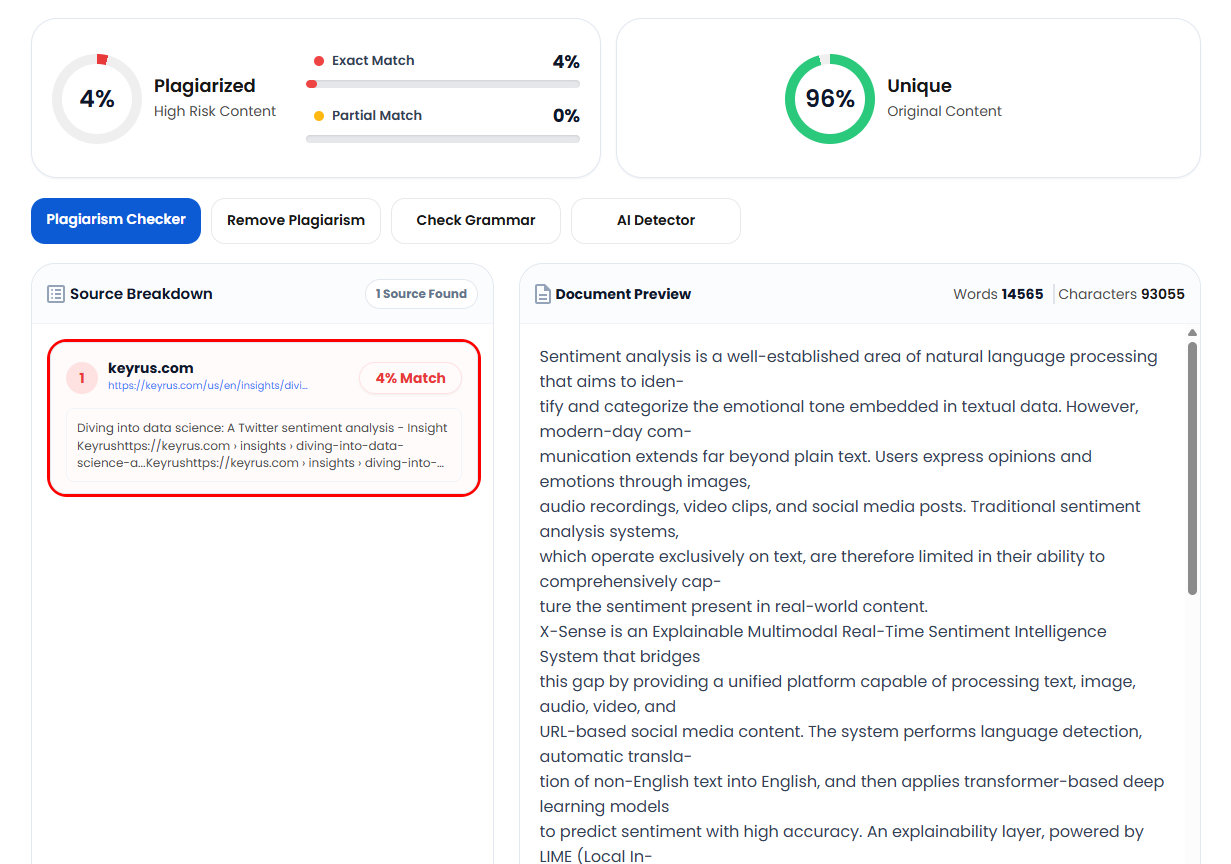
\includegraphics[width=\linewidth]{plagiarism.png}
    \caption{Plagiarism Report}
    \label{fig:plagiarism-report}
\end{figure}

\end{document}